\documentclass[a4paper,11pt]{article}
\pdfoutput=1 

\usepackage{jinstpub} 
\usepackage[utf8]{inputenc}
\usepackage{lineno}

\usepackage[capitalise,noabbrev,nameinlink]{cleveref}
\newlength{\abc}
\settowidth{\abc}{\space}
\AtBeginDocument{%
\renewcommand{\ref}[1]{\mbox{\Cref{#1}}}
\renewcommand{\equationautorefname}{Equation~\hspace{-\abc}}
\renewcommand{\sectionautorefname}{Section\,\negthinspace}
\renewcommand{\subsectionautorefname}{Section\,\negthinspace}
\renewcommand{\subsubsectionautorefname}{Section\,\negthinspace}
\renewcommand{\figureautorefname}{Figure\,\negthinspace}
\renewcommand{\tableautorefname}{Table\,\negthinspace}
}

% si units
\usepackage[binary-units=true]{siunitx}

% multirows in tables
\usepackage{multirow}

\usepackage{textcomp}
\usepackage{xcolor}
\usepackage{graphicx}
\usepackage{mathtools}
\usepackage{subcaption}
\usepackage[LGRgreek]{mathastext}
\usepackage{xspace}
%
% text handling
%

% vertical offset shortcut for paragraphs
\newcommand{\pg}[0]{\vspace*{0.75em}\newline}

% indentation shortcut
\newcommand{\ind}[0]{\hspace*{\customindent}}

% combination of vertical offset and indentation
\newcommand{\parag}{\parag\ind}


%
% content shorthands
%

% text and name highlights
\newcommand{\thl}[1]{``#1''}
\newcommand{\nhl}[1]{\textsc{#1}}

% missing citations
\newcommand{\tocite}[1]{\textbf{\textcolor{red}{[\ifthenelse{\equal{#1}{}}{?}{#1}]}}}

% arXiv and cds link
\newcommand{\arxivlink}[2]{\href{https://arxiv.org/abs/#1}{\texttt{arXiv:#1\,[#2]}}}
\newcommand{\cdslink}[1]{\href{http://cds.cern.ch/record/#1}{\texttt{cds:#1}}}

% argmin/max operators
\DeclareMathOperator*{\argmin}{arg\ min}
\DeclareMathOperator*{\argmax}{arg\ max}

% uneven plus-minus value
\newcommand{\upm}[4]{#1#2/\!#3\!#4}

%special signs
\newcommand{\inches}{\ensuremath{{}^{\prime\prime}}}
\newcommand{\skiroc}{SKIROC2-CMS}
\newcommand{\percent}{$\%$}
\newcommand{\permille}{\ensuremath{{}^\text{o}\mkern-5mu/\mkern-3mu_\text{oo}}}
\newcommand{\med}{\text{med}}

%% Units
\newcommand{\degrees}{\ensuremath{^{\circ}}\xspace}
\newcommand{\hitspermmbx}{\ensuremath{\text{Hits/mm}^{2}\text{/BX}}\xspace}
\newcommand{\permmbx}{\ensuremath{\text{/mm}^{2}\text{/BX}}\xspace}
\newcommand{\flux}{\ensuremath{\text{n_{eq}}/\text{cm}^{2}/\text{yr}}\xspace}
\newcommand{\neqcm}{\ensuremath{\mathrm{n_{eq}}/\mathrm{cm}^{2}}\xspace}
\newcommand{\percms}{\ensuremath{\text{cm}^{-2}\mathrm{s}^{-1}}\xspace}
\newcommand{\micron}{\ensuremath{\upmu\mathrm{m}}\xspace}
\newcommand{\microsecond}{\ensuremath{\upmu\mathrm{s}}\xspace}
\newcommand{\microwatt}{\ensuremath{\upmu\mathrm{W}}\xspace}

%abbreviations
\newcommand{\eg}{e.g.}
\newcommand{\ie}{i.e.}

%software
\newcommand{\CMSSW}{\textsc{CMSSW}}
\newcommand{\ROOT}{\textsc{ROOT}}
\newcommand{\corryvreckan}{\textsc{CORRYVRECKAN}}
\newcommand{\Geant}{\textsc{GEANT4}}
\newcommand{\luigi}{\textsc{LUIGI}}
\newcommand{\millepede}{\textsc{MILLEPEDE}}

%
% physics processes
%

\newcommand{\slep}{\text{single-lepton}}
\newcommand{\dlep}{\text{dilepton}}
\newcommand{\fullh}{\text{full-hadron}}
\newcommand{\Slep}{\text{Single-lepton}}
\newcommand{\Dlep}{\text{Dilepton}}
\newcommand{\Fullh}{\text{Full-hadron}}
\newcommand{\slepe}{\text{single-electron}}
\newcommand{\slepmu}{\text{single-muon}}
\newcommand{\Slepe}{\text{Single-electron}}
\newcommand{\Slepmu}{\text{Single-muon}}

\newcommand{\hf}{\text{heavy-flavor}}
\newcommand{\ttbar}{\ensuremath{t\bar{t}}}
\newcommand{\bbbar}{\ensuremath{b\bar{b}}}
\newcommand{\ccbar}{\ensuremath{c\bar{c}}}
\newcommand{\totbar}{\ensuremath{t\hspace{-0.5mm}/\hspace{-0.5mm}\bar{t}}}
\newcommand{\bobbar}{\ensuremath{b\hspace{-0.5mm}/\hspace{-0.5mm}\bar{b}}}
\newcommand{\ttH}{\ensuremath{\ttbar H}}
\newcommand{\Hbb}{\ensuremath{H\rightarrow \bbbar}}
\newcommand{\Hnbb}{\ensuremath{H\nrightarrow \bbbar}}
\newcommand{\HWW}{\ensuremath{H\rightarrow W^+W^-}}
\newcommand{\Htautau}{\ensuremath{H\rightarrow \tau^+\tau^-}}
\newcommand{\ttHbb}{\ensuremath{\ttH\,(\Hbb)}}
\newcommand{\ttHnbb}{\ensuremath{\ttH\,(\Hnbb)}}
\newcommand{\ttX}{\ensuremath{\ttbar\!+\!\text{X}}}
\newcommand{\ttbb}{\ensuremath{\ttbar\!+\!\bbbar}}
\newcommand{\ttb}{\ensuremath{\ttbar\!+\!\bobbar}}
\newcommand{\tttb}{\ensuremath{\ttbar\!+\!2b}}
\newcommand{\ttcc}{\ensuremath{\ttbar\!+\!\ccbar}}
\newcommand{\ttlf}{\ensuremath{\ttbar\!+\!\text{lf}}}
\newcommand{\tthf}{\ensuremath{\ttbar\!+\!\text{hf}}}
\newcommand{\Singlet}{\ensuremath{\text{Single}\ \totbar}}
\newcommand{\singlet}{\ensuremath{\text{single}\ \totbar}}
\newcommand{\Singlett}{\ensuremath{\text{Single}\ t}}
\newcommand{\Singletbar}{\ensuremath{\text{Single}\ \bar{t}}}
\newcommand{\Vjets}{\ensuremath{V\hspace{-0.5mm}\!+\!\text{jets}}}
\newcommand{\Wjets}{\ensuremath{W\hspace{-0.5mm}\!+\!\text{jets}}}
\newcommand{\Zjets}{\ensuremath{Z\hspace{-0.5mm}\!+\!\text{jets}}}
\newcommand{\Diboson}{\ensuremath{\text{Diboson}}}
\newcommand{\diboson}{\ensuremath{\text{diboson}}}
\newcommand{\ttW}{\ensuremath{\ttbar\!+\!W}}
\newcommand{\ttZ}{\ensuremath{\ttbar\!+\!Z}}
\newcommand{\ttV}{\ensuremath{\ttbar\!+\!V}}


%
% physics process colors
%

\definecolor{ttHcol}{RGB}{67,118,201}
\definecolor{ttbbcol}{RGB}{235,230,10}
\definecolor{ttbcol}{RGB}{205,0,10}
\definecolor{tttbcol}{RGB}{255,153,1}
\definecolor{ttcccol}{RGB}{131,38,10}
\definecolor{ttlfcol}{RGB}{81,142,25}
\definecolor{Singletcol}{RGB}{0,204,204}
\definecolor{Vjetscol}{RGB}{104,140,140}
\definecolor{Dibosoncol}{RGB}{1,25,147}
\definecolor{ttVcol}{RGB}{255,102,101}


%
% other physics variables
%

\newcommand{\BR}{\ensuremath{B\!R}}
\newcommand{\met}{\ensuremath{\cancel{E}_T}}
\DeclareRobustCommand{\orderof}{\ensuremath{\mathcal{O}}}


\title{\boldmath Electrical Characterisation of Silicon Pad Sensors Irradiated at the Rhode Island Nuclear Reactor for the CMS Endcap Calorimeter Upgrade}


\author[a]{Nick Hinton}
\author[b]{Timo Peltola}
\author[c]{Thorben Quast}
\author[c]{Eva Sicking}

\affiliation[a]{Brown University}
\affiliation[b]{Texas Tech University}
\affiliation[c]{CERN Experimental Physics Department}

\collaboration[d]{on behalf of the CMS HGCAL silicon group}

\emailAdd{thorben.quast@cern.ch}

\abstract{
    Electric characteristics of prototype sensors foreseen for the CMS calorimeter endcap after neutron irradiation at RINSC 2020-21 have been characterised and the empiric findings are presented in this paper.\newline\newline
} 
\keywords{Calorimeter, CMS, HGCAL, silicon sensors, neutron irradiation}

\linenumbers

\begin{document}
\maketitle
\flushbottom

\linenumbers
\section{Introduction}
\label{sec:introduction}
\textcolor{red}{Todo.}\newline

% The Large Hadron Collider at CERN will be upgraded to provide more instantaneous luminosity~\cite{hllhc-tdr:2017}.
% Experiments, such as CMS, need to upgrade their detector systems. 
%One of the CMS upgrades is the replacement of the current endcap calorimeters with the High Granularity Calorimeter (HGCAL)~\cite{hgcal-tdr:2018}.
% Silicon sensors will be used and their electrical properties are important to assess after irradiation.
% This is what we will show here.
% Exposing silicon sensors to radiation introduces defects in the bulk and with it worsens their electrical properties in view of their application as particle detectors.
% In particular, the bulk-dominated leakage current density is expected to increase proportionally with the fluence, and sensors are expected to deplete at higher bias voltages with increasing fluence levels.
% Annealing can cure radiation-induced defects to some extent, hereby reducing the degradation of the leakage current and the depletion voltage.
\section{Prototype Silicon Sensors for CMS Endcap Calorimeter Upgrade}
\label{sec:sensors}

\begin{itemize}
    \item Explain common parameters
    \item Explain different production parameters
    \item Define grading critera / expectations
\end{itemize}
\section{Neutron Irradiation}
\label{sec:irradiation}

\subsection{Rhode Island Neutron Irradiation Facility}
\label{subsec:RINSC}
RINSC (Rhode Island Nuclear Science Center) is a 2 MW, light water cooled, pool type reactor in Narragansett, Rhode Island, USA.
The core consists of fuel assemblies reflected with a combination of graphite and beryllium.
The fuel is plate type U3Si2 cladded with aluminum enriched to less than 20% Uranium-235.
At RINSC there are three (technically six, do we only include the ones we use?) different ways to irradiate materials: beamports (pipes that run from the work area to the reactor core), rabbit system (pneumatic system that ferries plastic sample bottles to the reactor core), and InCore tubes (small samples are placed into a tube and lowered into an empty basket next to the fuel elements). 
The beamports can accomodate samples of up to 7.75" x 3' [diameter by length], the rabbit system can accept sampes 1.125" x 6.25", and the InCore system can irradiate objects 1.25" x 9". 
Of the irradiation methods available, only the beamports are large enough to accomodate the silicon sensors for this project.
\begin{itemize}
    \item Fig 1 - image(s) of reactor core, beamport (see figure~\ref{fig:RINSC_Facility})
    what other details are useful here?
    Is it better to omit the sample irradiation options that are not being used?
    \item Fig 2 - puck design/layout, real pucks (see figure~\ref{fig:Pucks_Arrayed})
    \item Fig 3 - puck layout, packing (see figure~\ref{fig:Puck_Packing}), how much detail about packing materials? (see figure~\ref{fig:Cylinder_Details})
    \item Fig 4 - other hardware, cylinder, temp monitoring setup (see figure~\ref{fig:Temperature_Monitoring_Setup})
    Keithley 2400 for temperature readout (along with 20-channel input board), RTDs instrumented with 20' of radiation-resistant wire (McMaster), laptop with GPIB connection to keithely, and custom LabVIEW code for readout.
    \item Fig 5 - schemaitc of experimental setup? Is this needed?
    \item describe sample removal/storage after irradiation - need for full day for activity levels to decay to the point that reactor staff can transfer cylinder from beamport to freezer. Chest freezer has been installed a few steps away from the beamport with enough storage capacity for 3 cylinders.
    \item Fig 6 describe fluence measurement setup/procedure at Brown? IV of D0 diodes prior to irradiation, then cold (-20C) measurement of irradiated diodes with current scaled up to 20C. Also include pin diodes but they have not been found to be useful at fluences above 1e15. (see figure~\ref{fig:Fluence_Measurement_Setup})
\end{itemize}

\begin{figure}[!hbt]
  \begin{center}
    \includegraphics[width=0.25\textwidth]{figures/RINSC_Reactor_Core}
    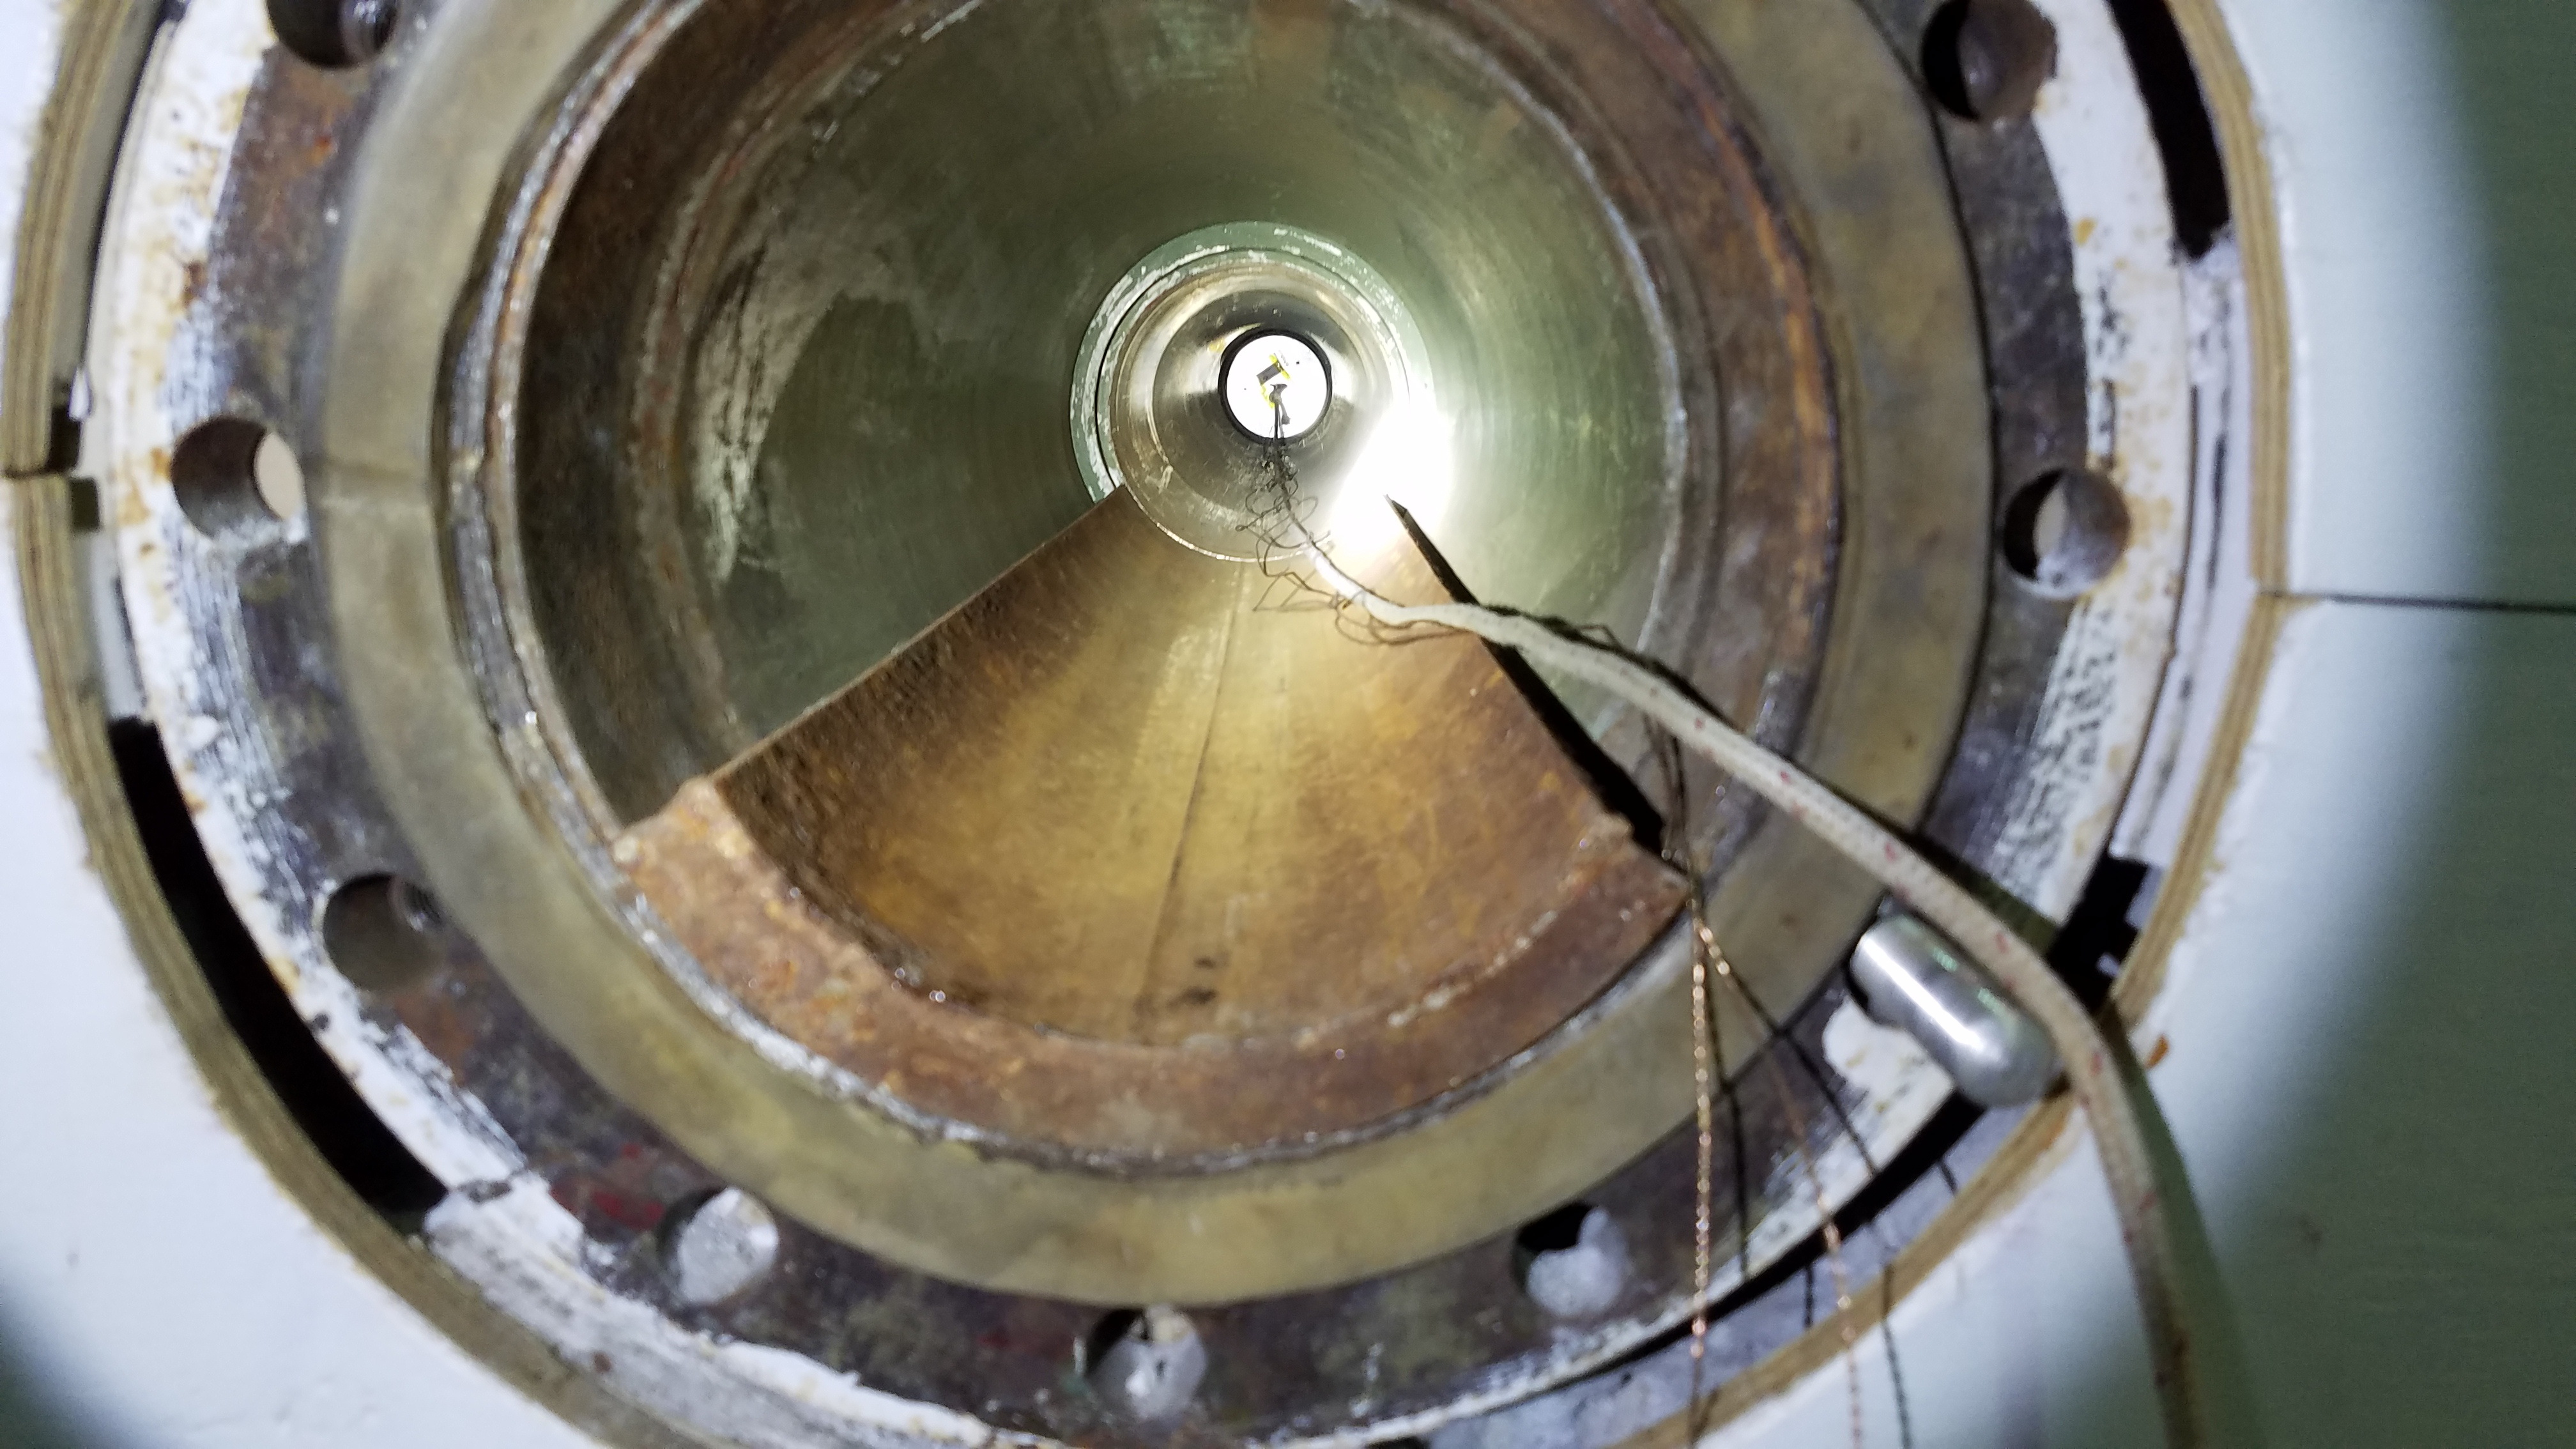
\includegraphics[width=0.40\textwidth]{figures/Beamport_View}
    \caption{On the left is an image of the reactor core at RINSC, and on the right is a view down the beamport used for these irradiation studies.}
    \label{fig:RINSC_Facility}
  \end{center}
\end{figure}

\begin{figure}[!hbt]
  \begin{center}
    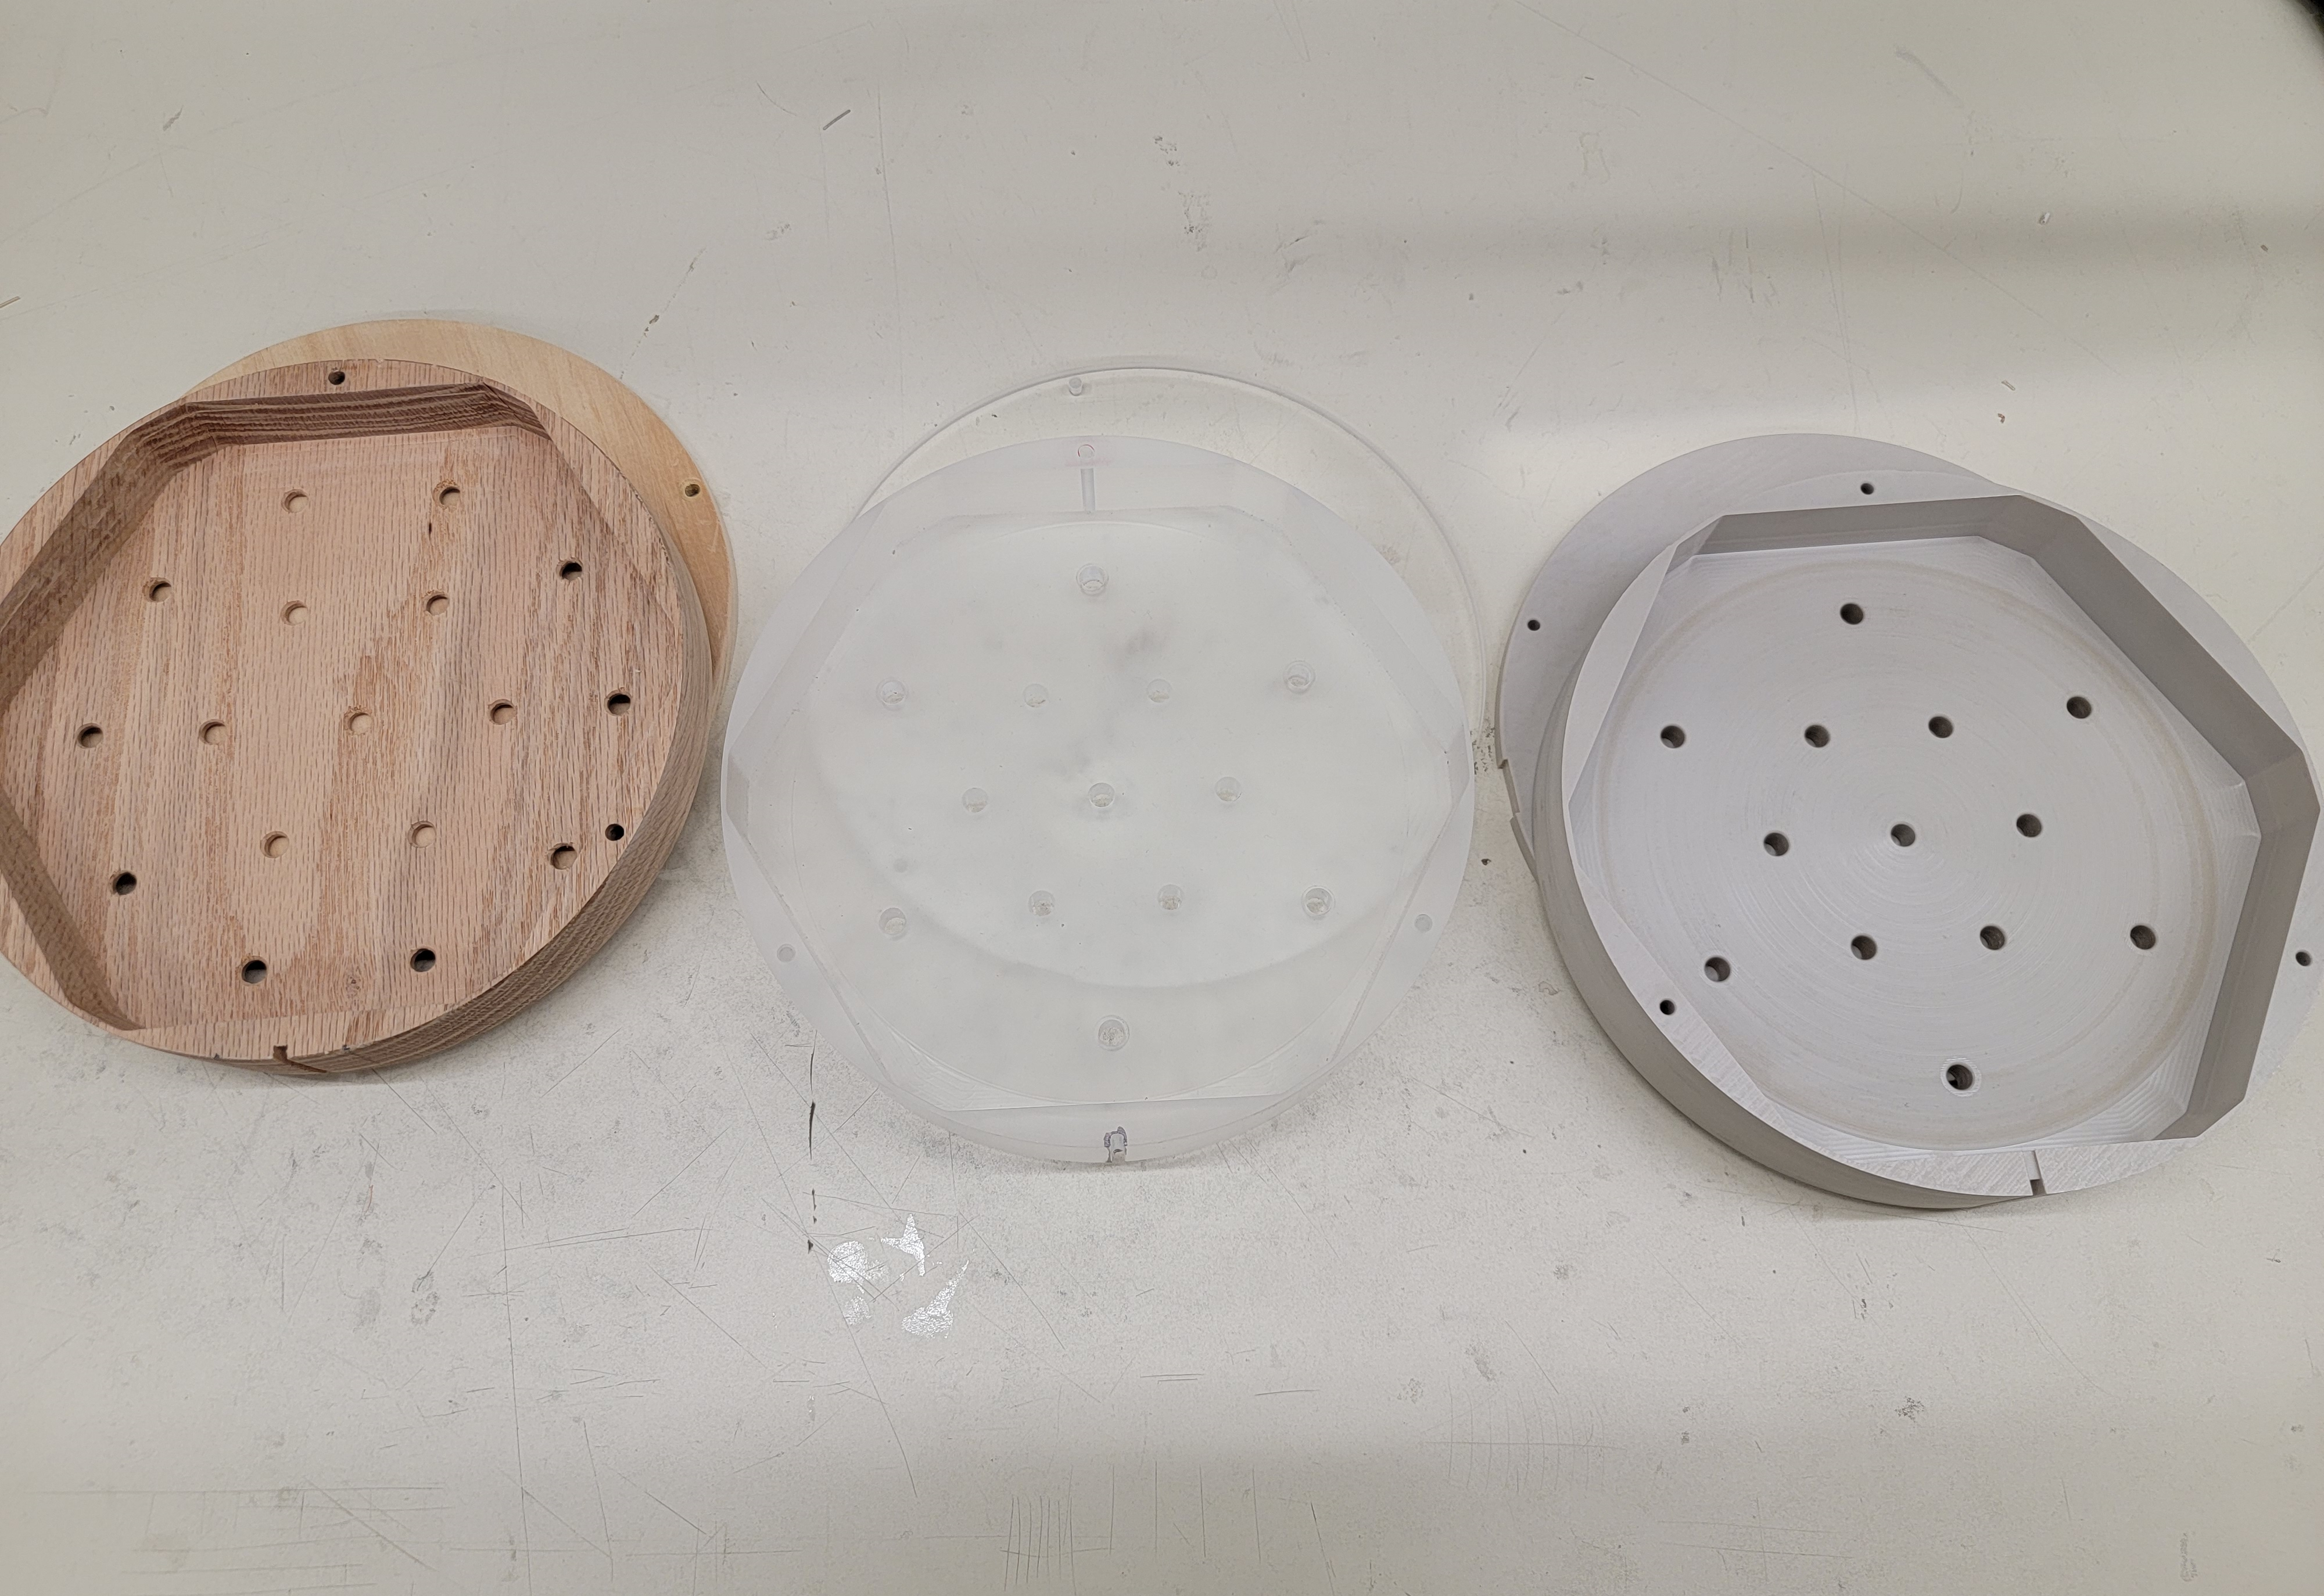
\includegraphics[width=0.70\textwidth]{figures/Hockey_Pucks_Arrayed}
    \caption{Sample containers ('hockey pucks') for sensors to be irradiated in the beamport at RINSC. The materials are wood (oak), acrylic, and PEEK.}
    \label{fig:Pucks_Arrayed}
  \end{center}
\end{figure}

\begin{figure}[!hbt]
  \begin{center}
    \includegraphics[width=0.70\textwidth]{figures/Cylinder_Side_View}
    \includegraphics[width=0.70\textwidth]{figures/Cylinder_With_Dry_Ice}
    \caption{Left: aluminum cylinder used to transport hockey puck containers into the beamport. Right: cylinder containing a sample puck along with dry ice for cooling.}
    \label{fig:Cylinder_Details}
  \end{center}
\end{figure}

\begin{figure}[!hbt]
  \begin{center}
    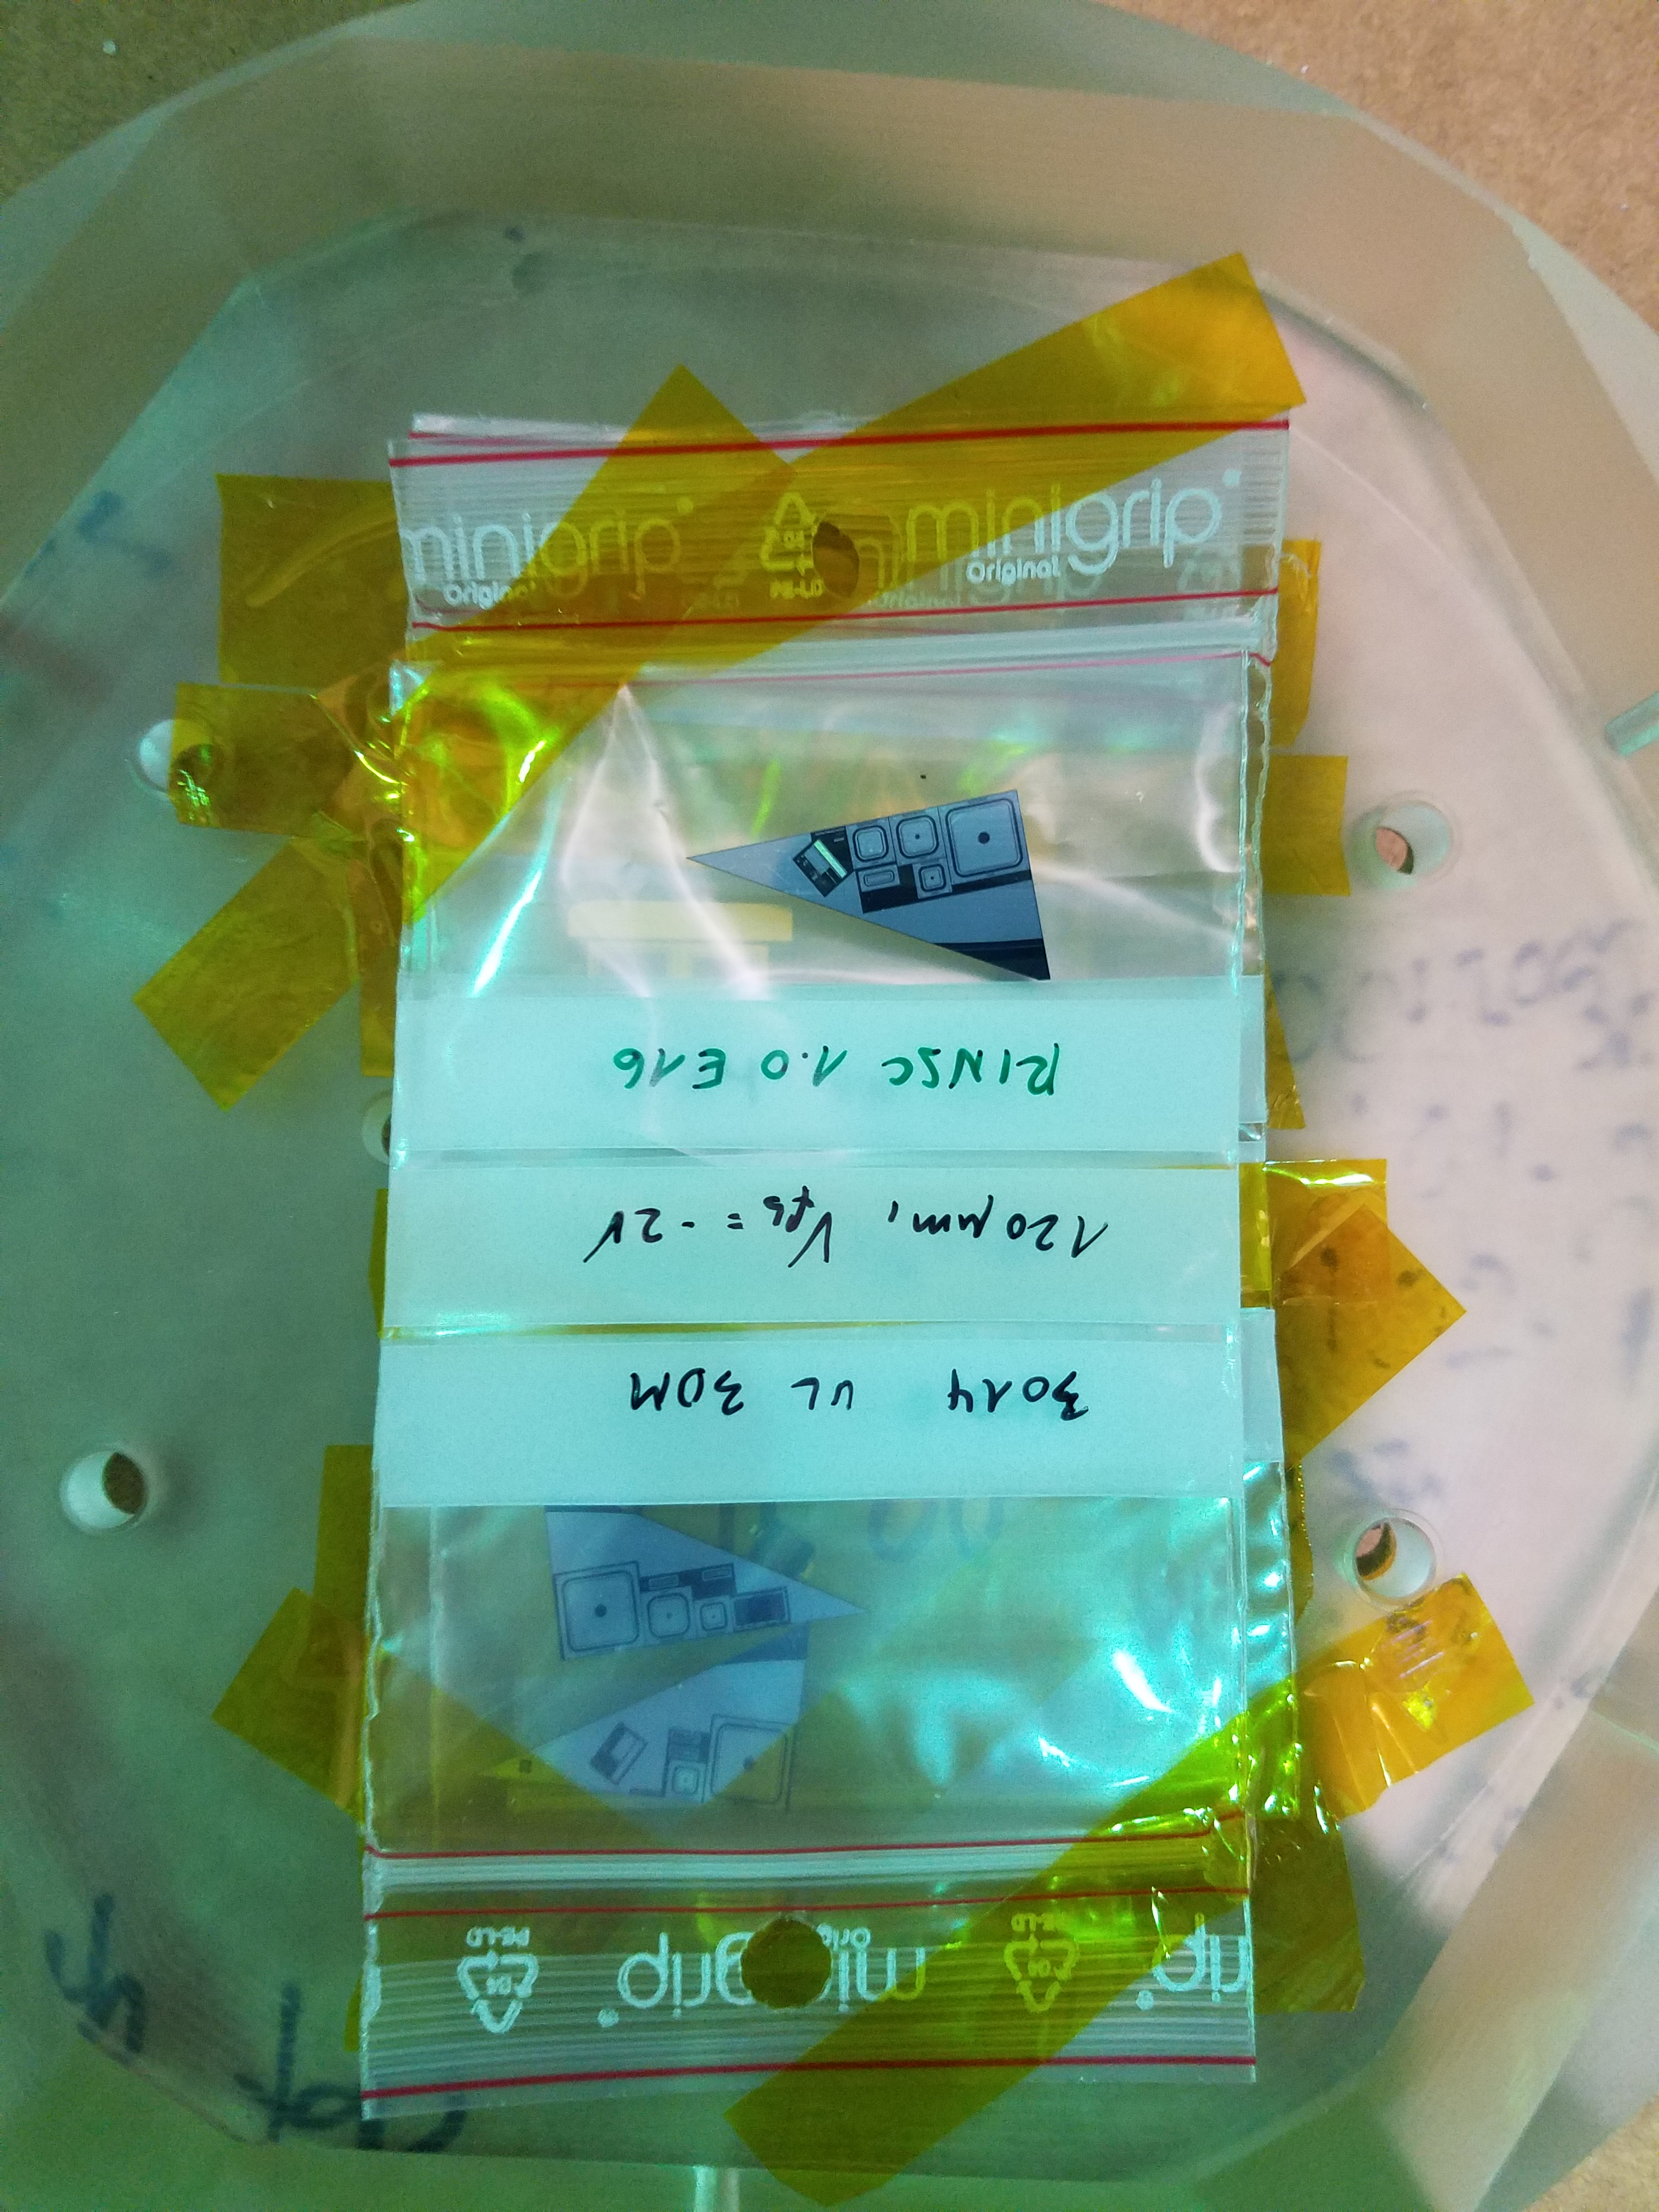
\includegraphics[width=0.20\textwidth]{figures/Hockey_Puck_Base_Instrumented}  
    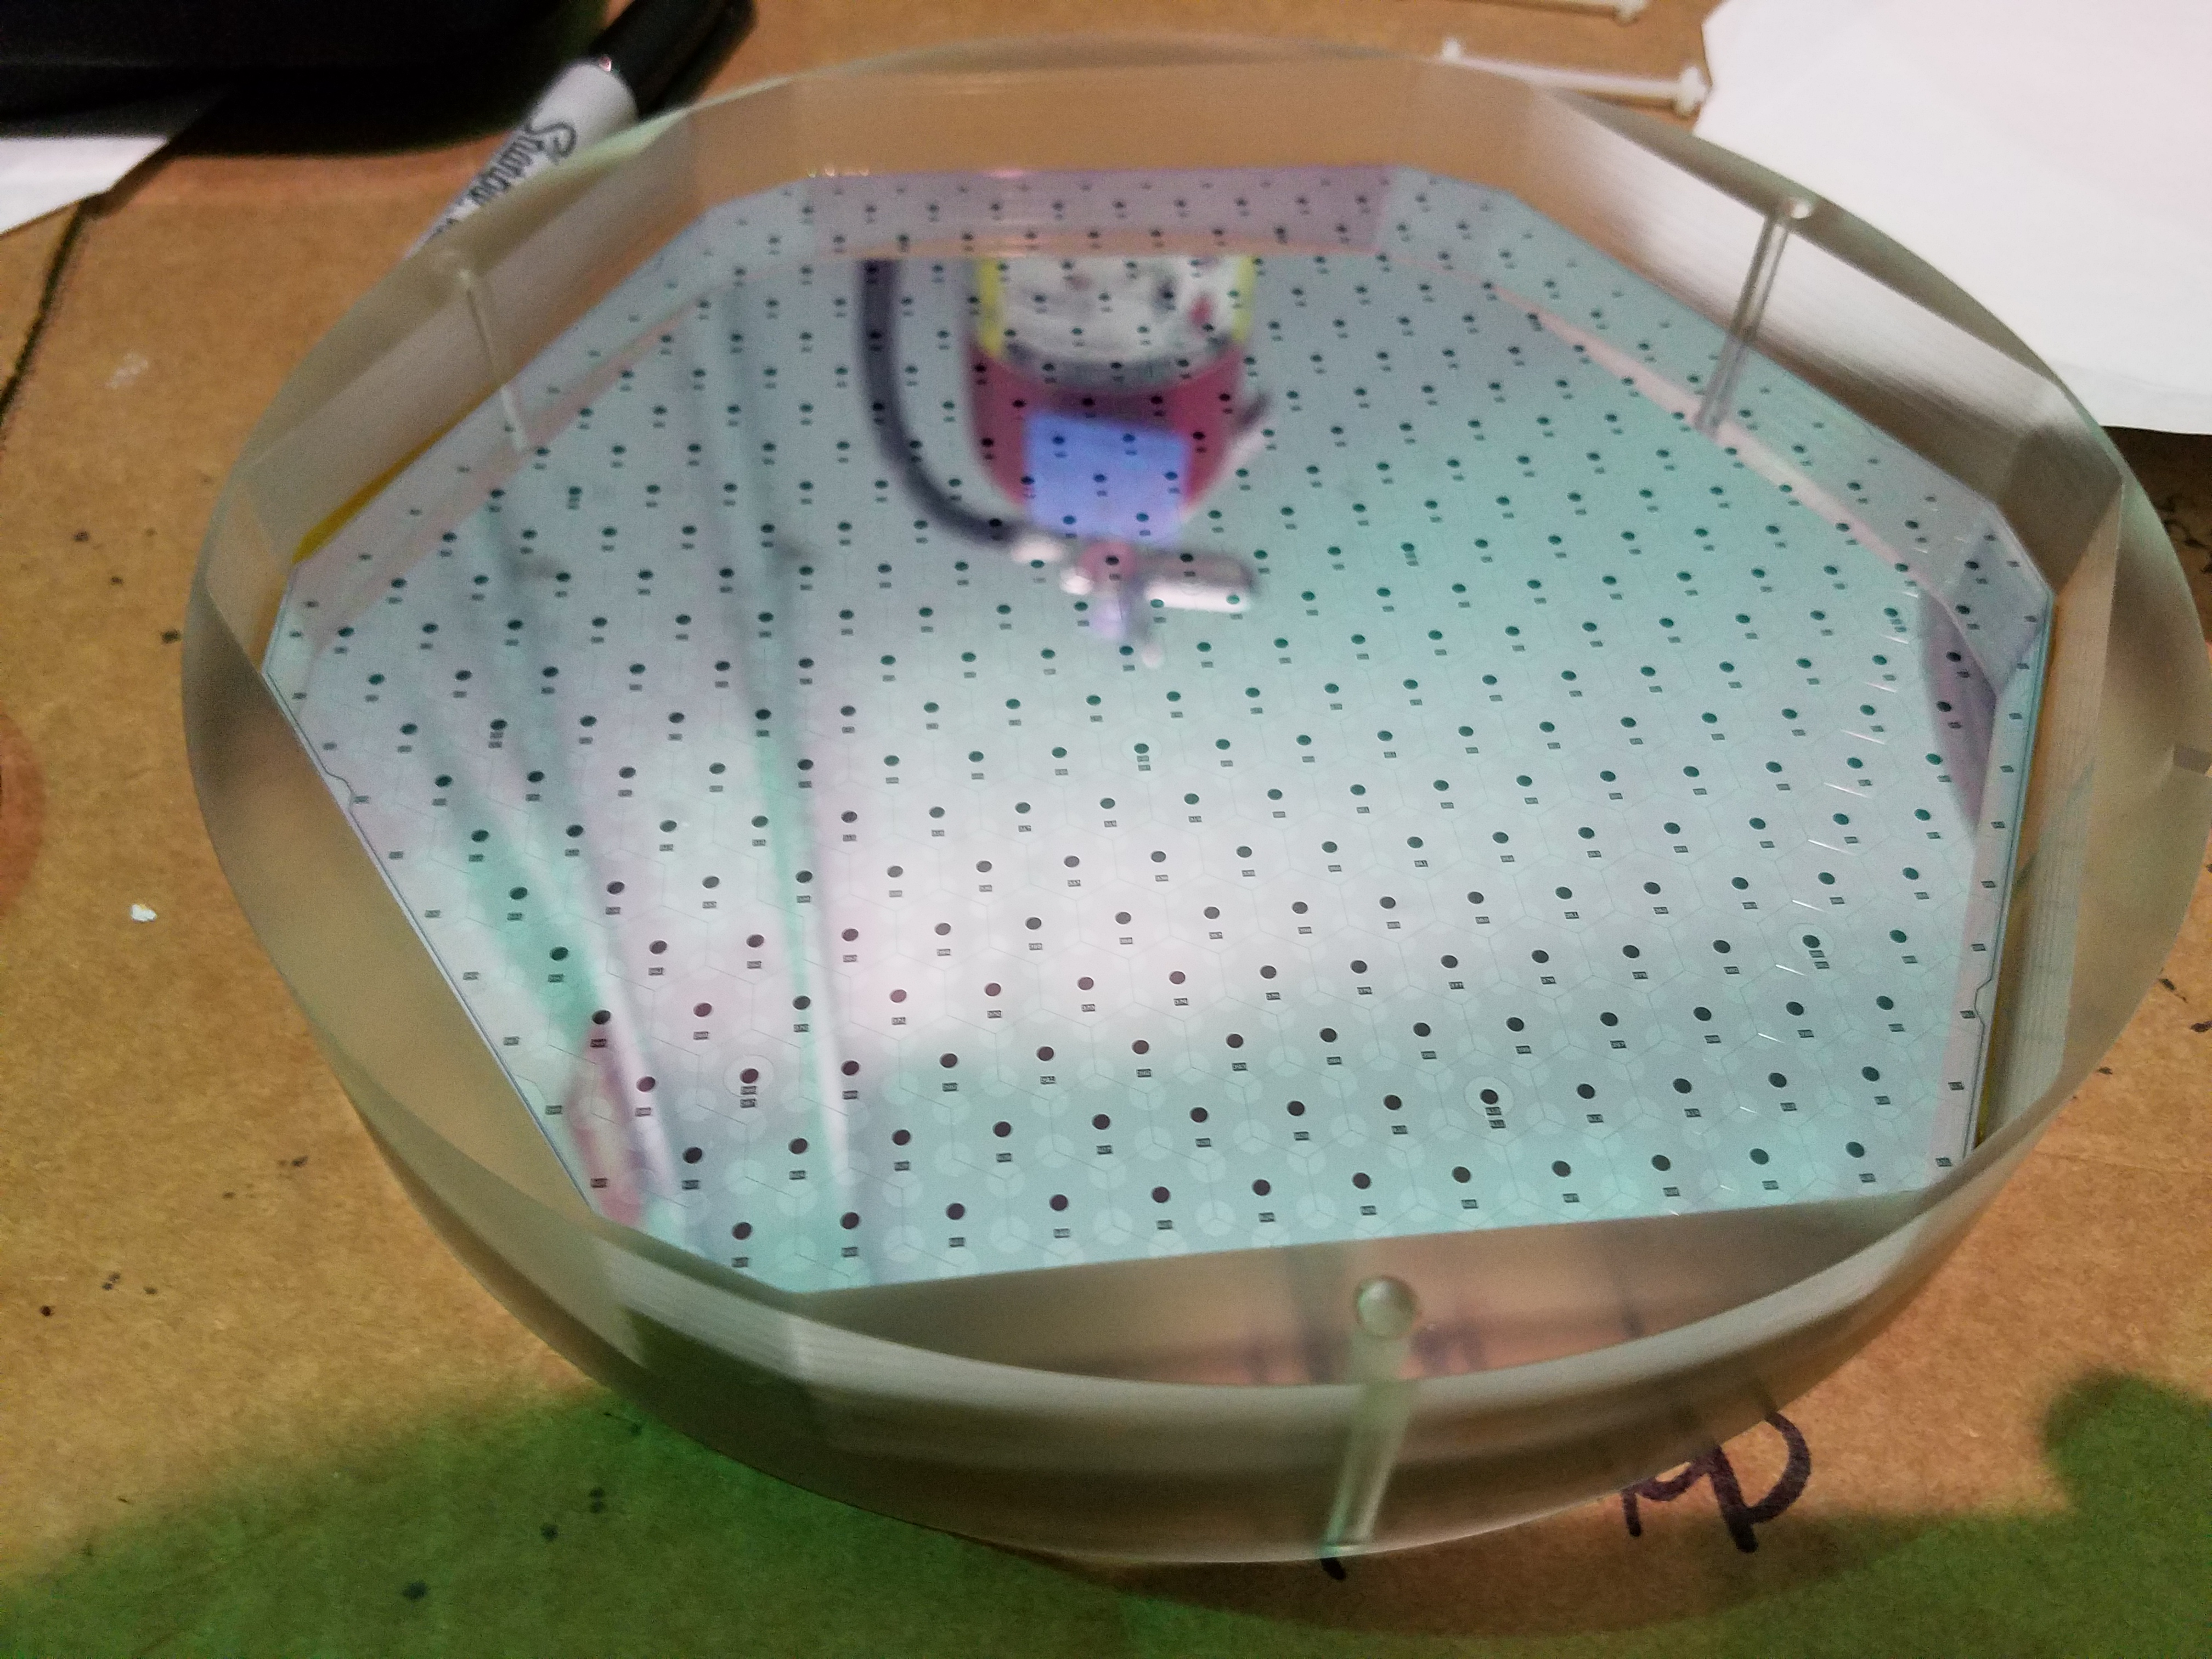
\includegraphics[width=0.25\textwidth]{figures/Hockey_Puck_Sensor_Fit}
    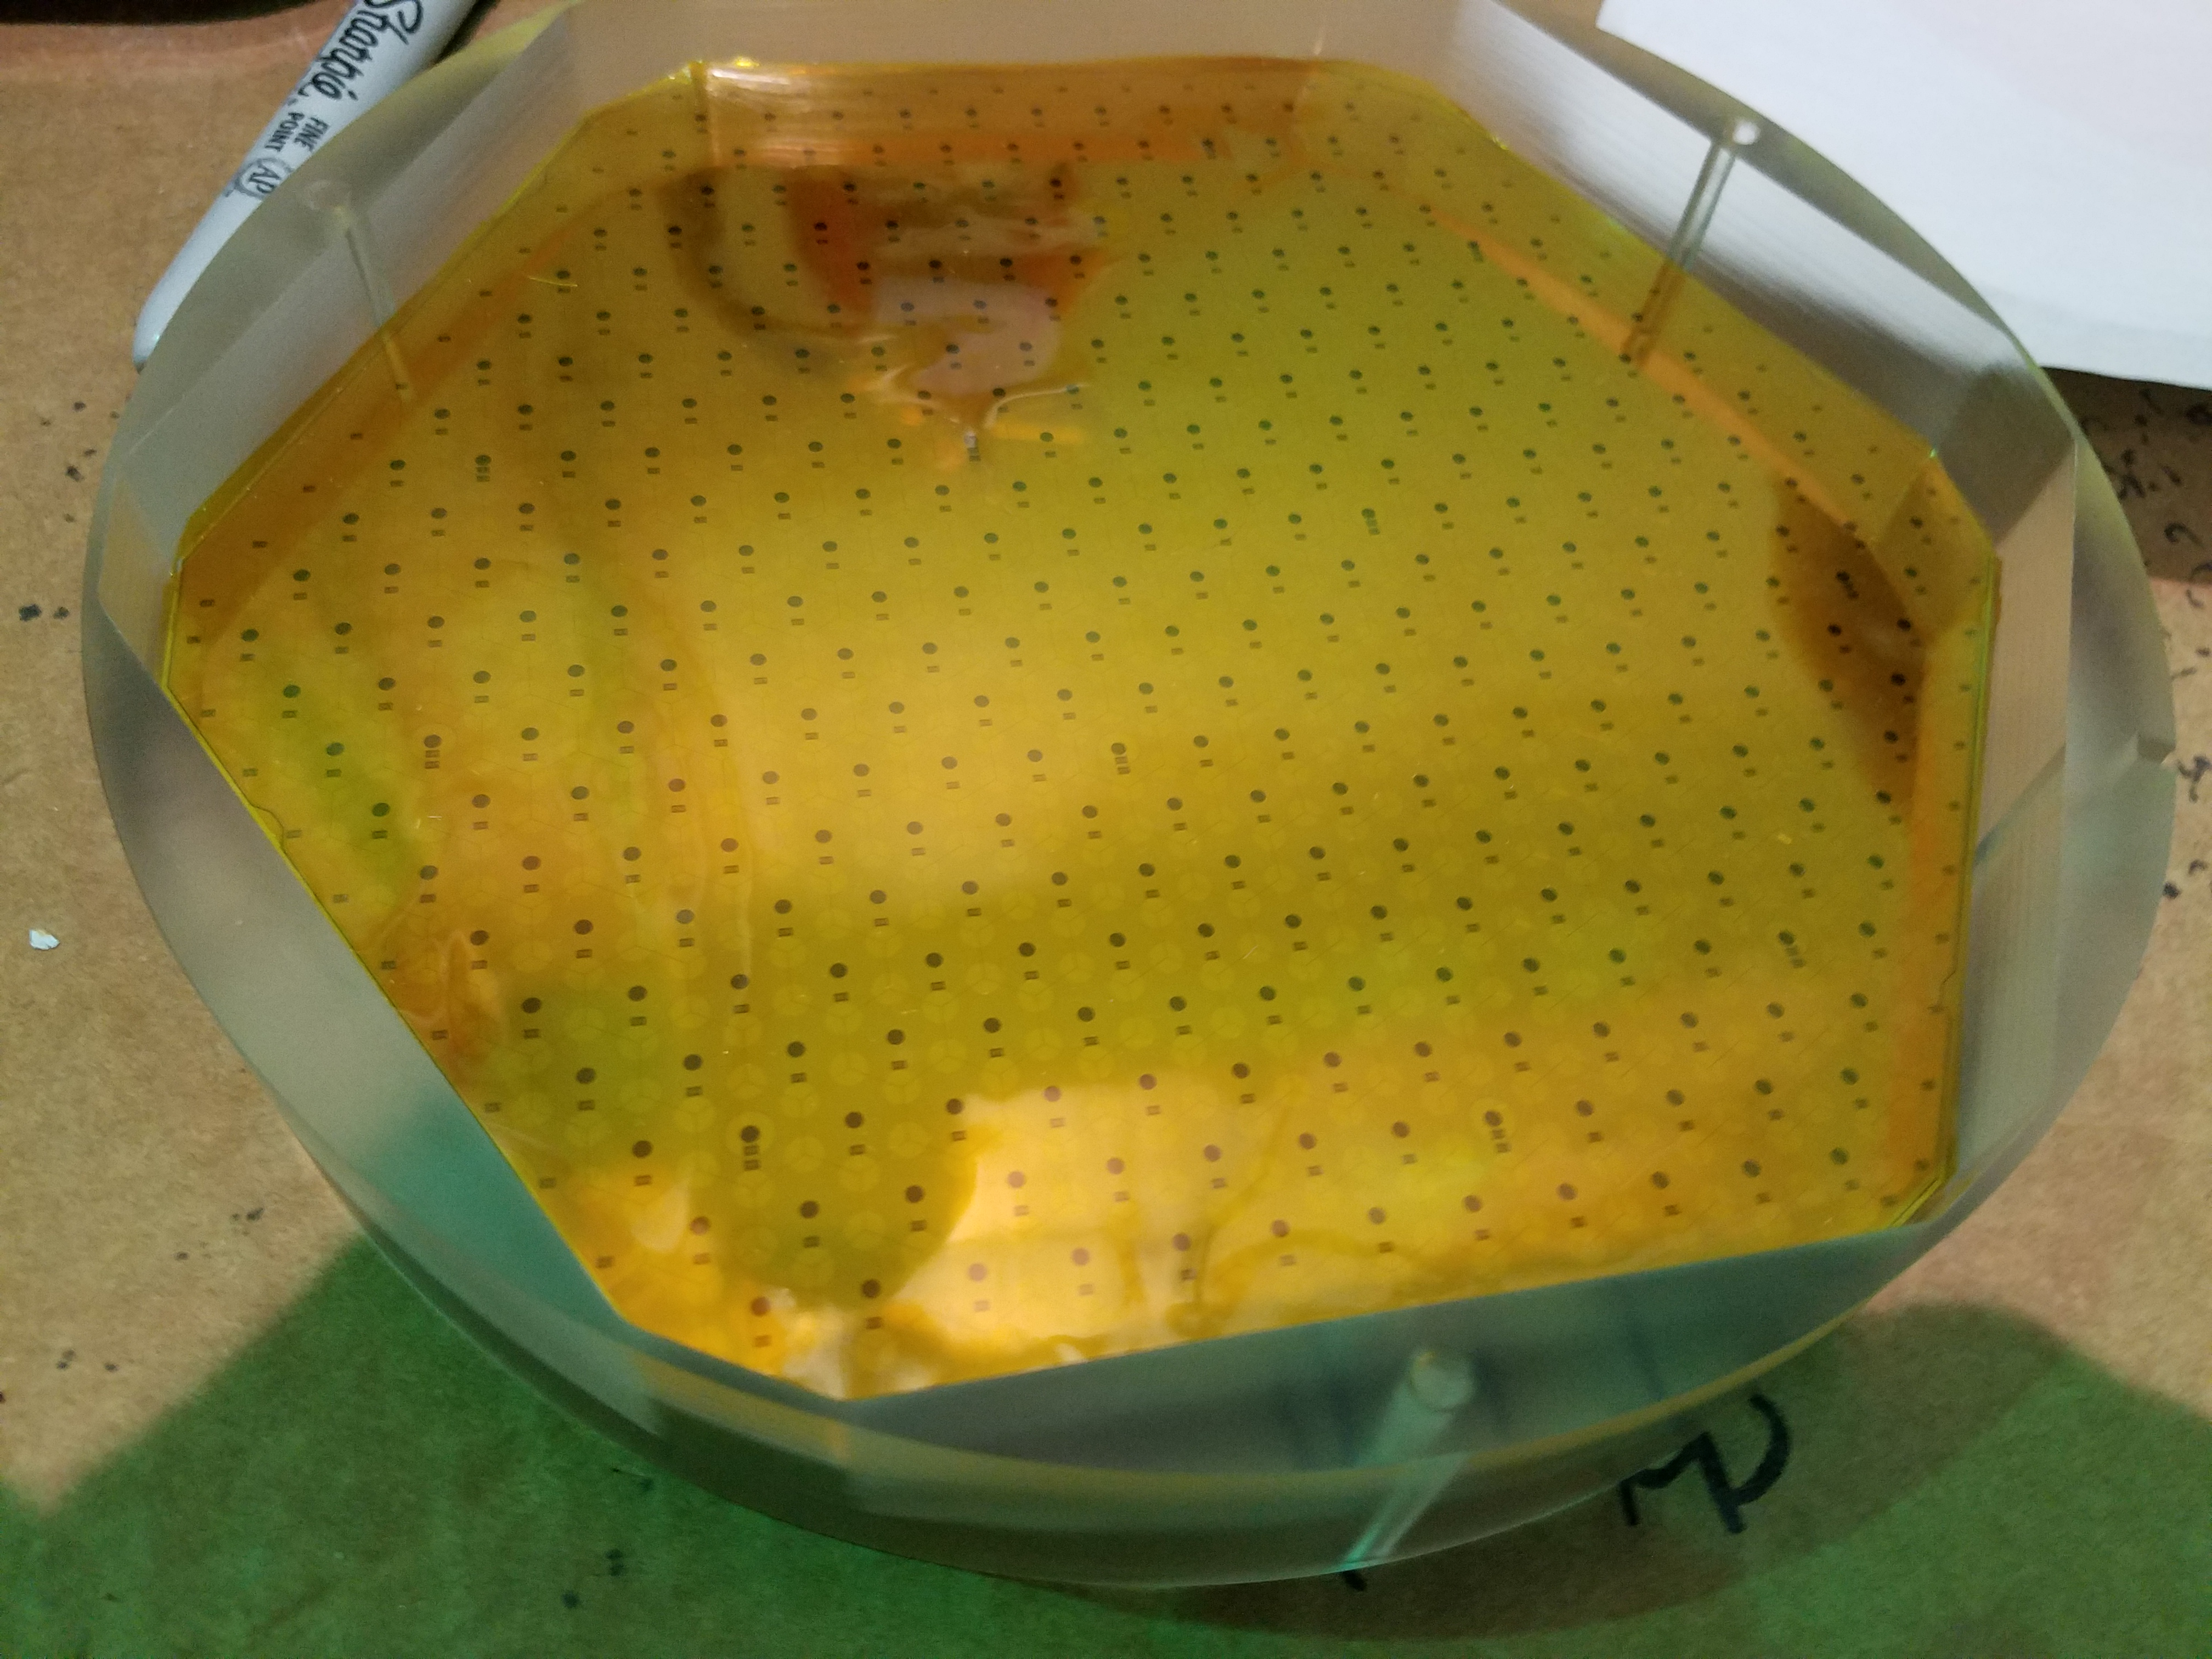
\includegraphics[width=0.25\textwidth]{figures/Hockey_Puck_Kapton_Layer}
    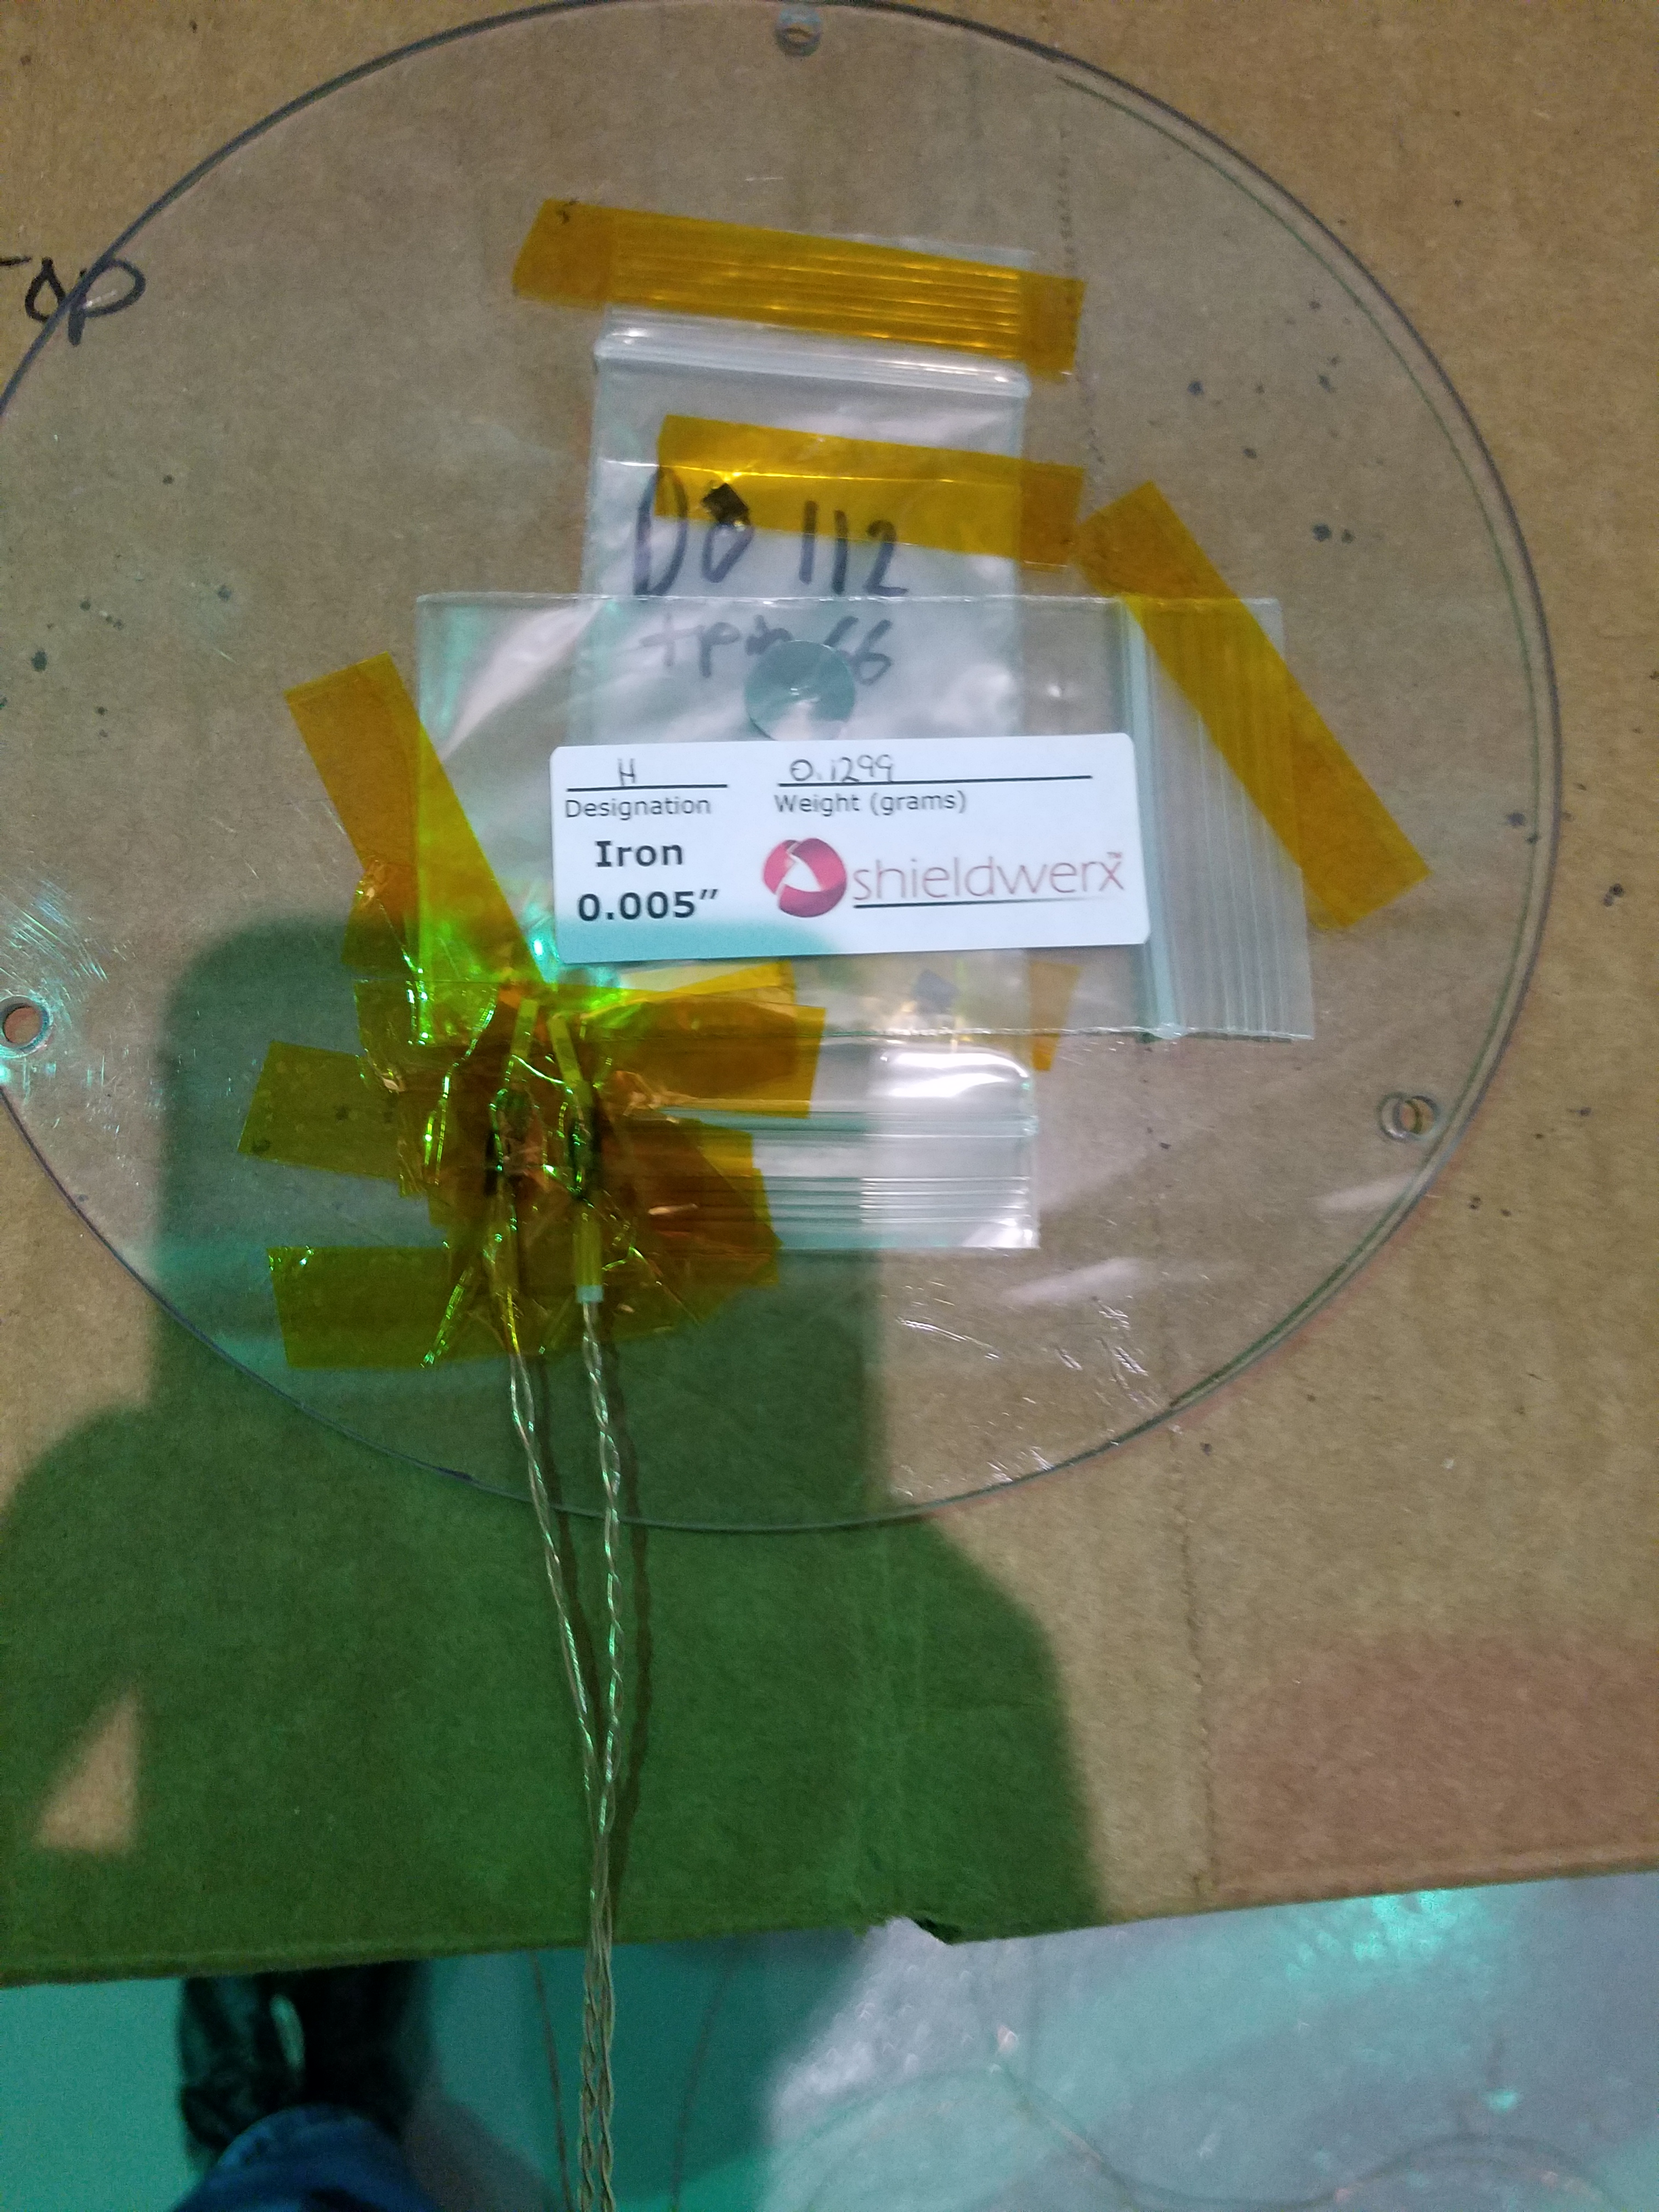
\includegraphics[width=0.20\textwidth]{figures/Hockey_Puck_Lid_Instrumented}    
    \caption{Four views of sensor container packing: the base instrumented with fluence monitoring diodes, the fit of a sensor in the hockey puck, the protection of the sensor with layers of kapton foil, and the lid of the hockey puck instrumented with monitoring devices.}
    \label{fig:Puck_Packing}
  \end{center}
\end{figure}

\begin{figure}[!hbt]
  \begin{center}
    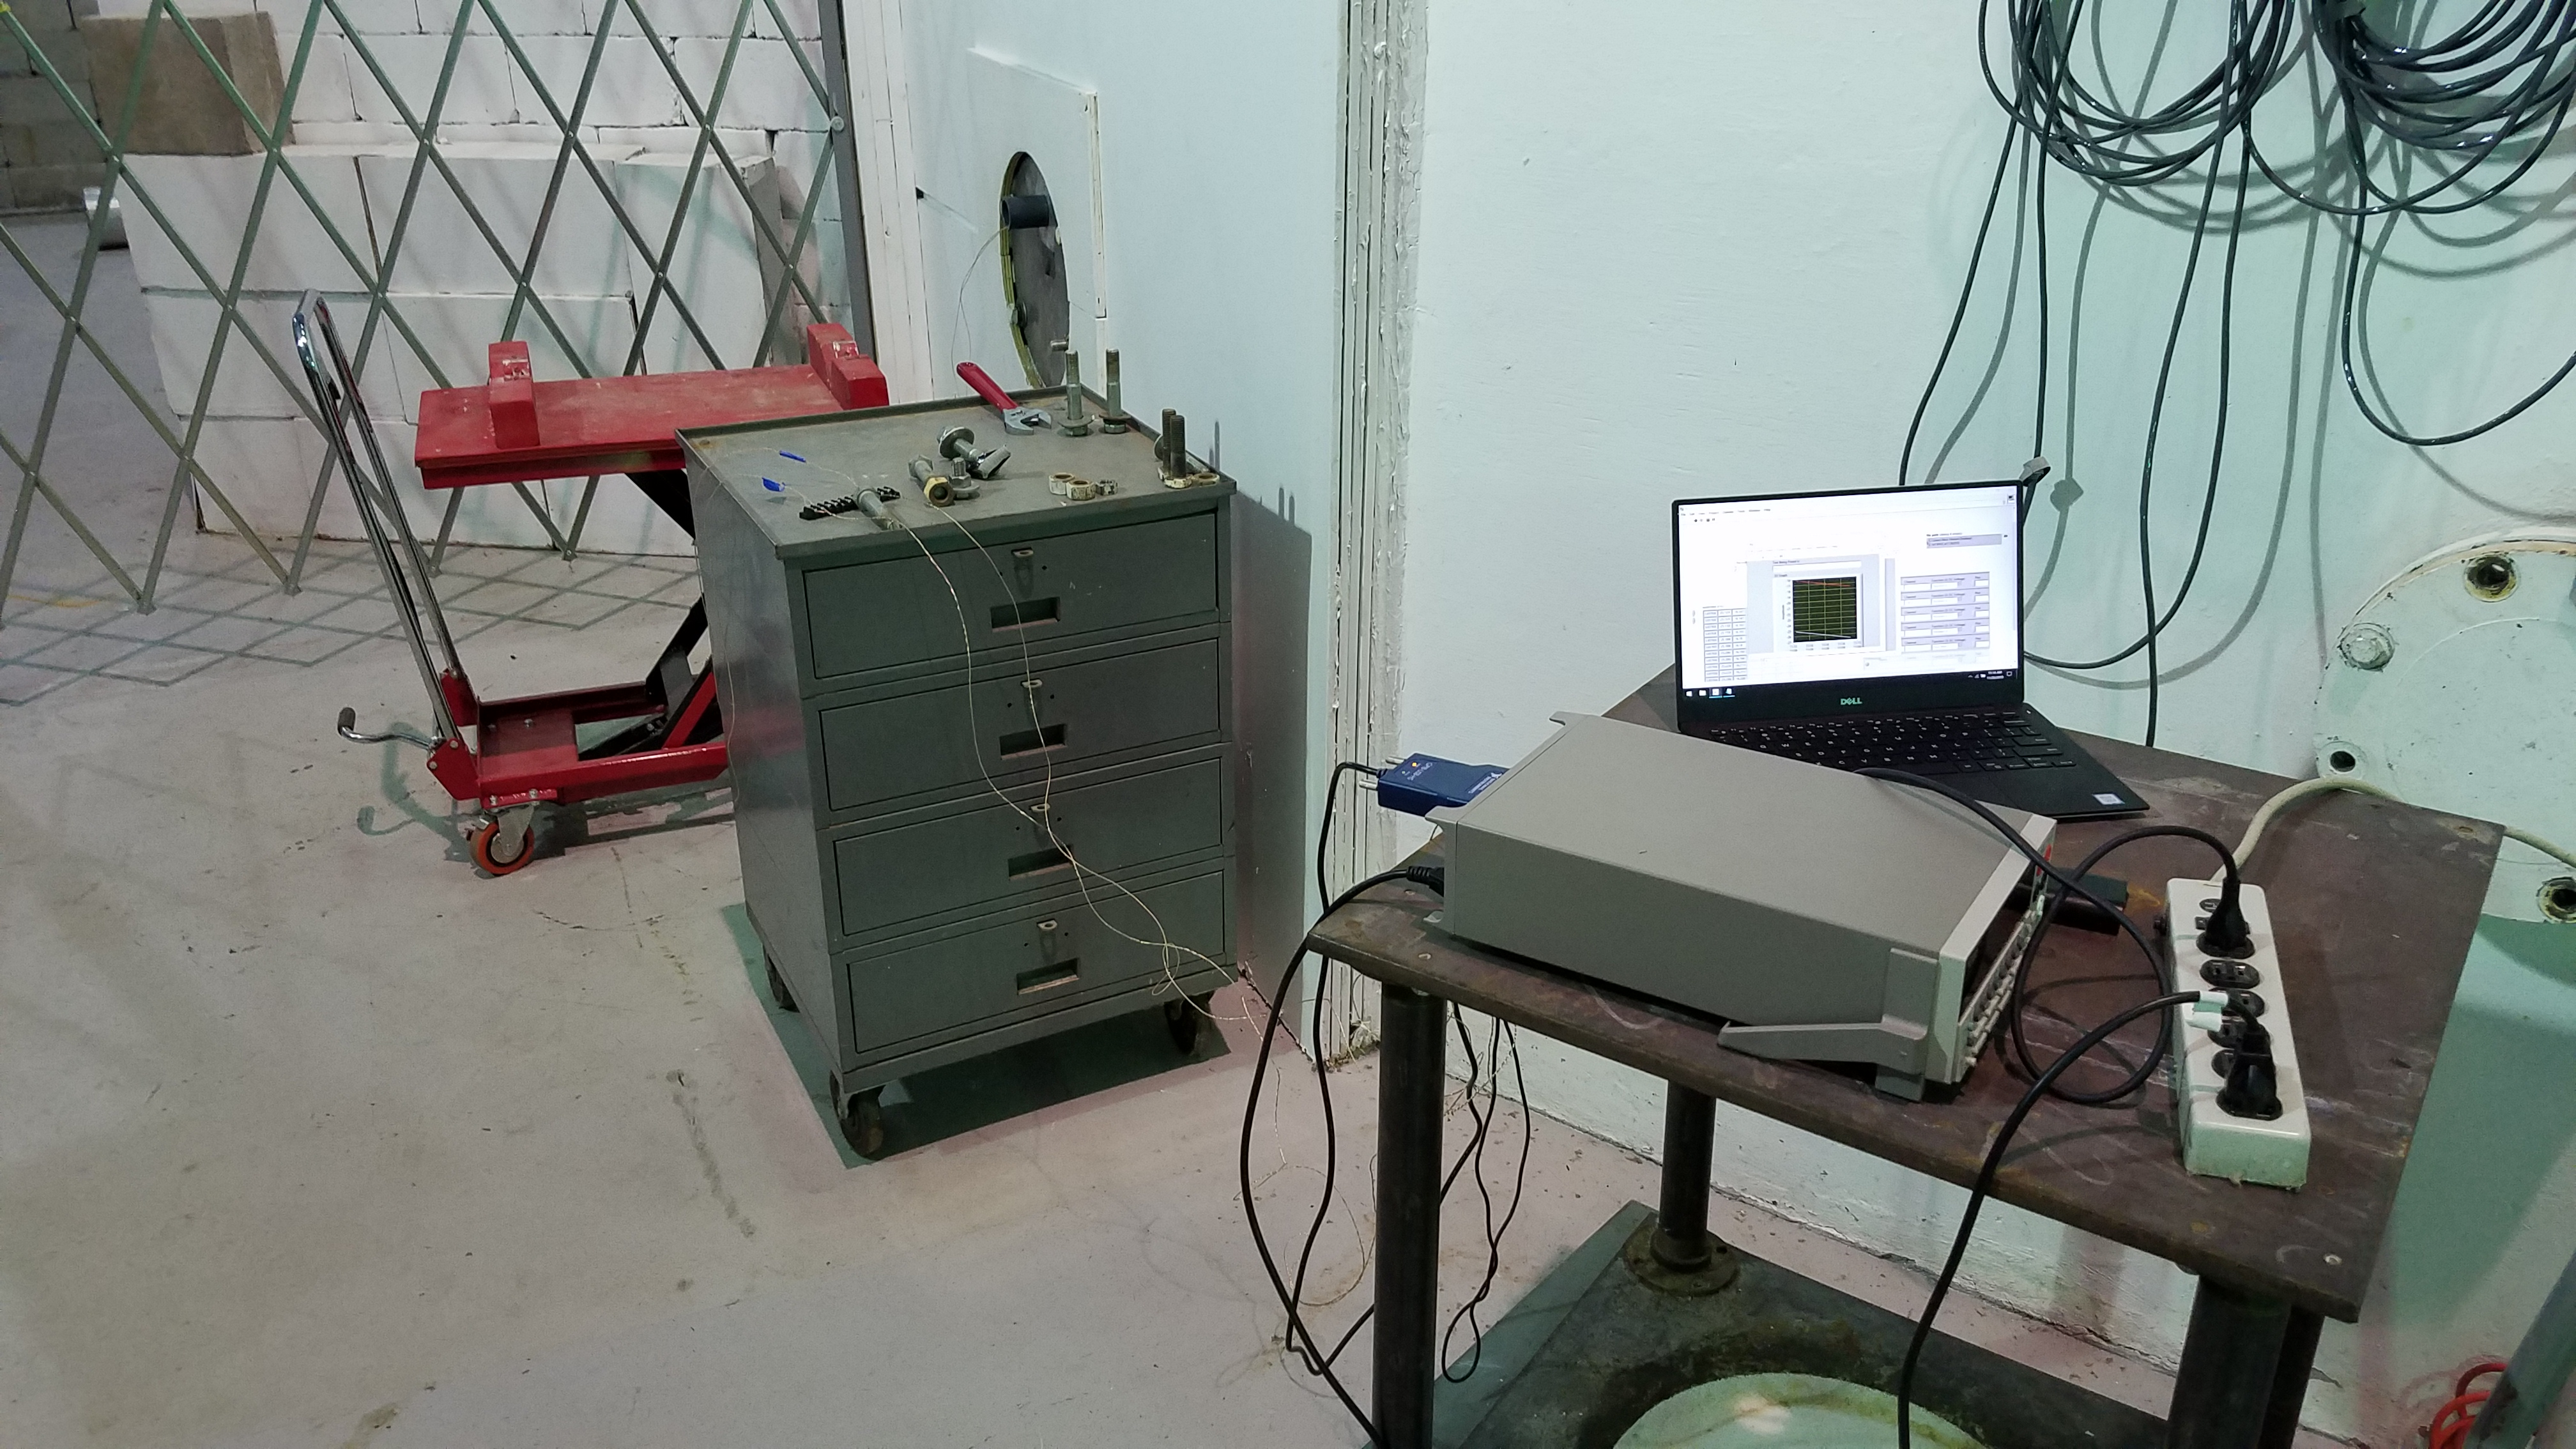
\includegraphics[width=0.80\textwidth]{figures/Temperature_Monitoring_Setup}
    \caption{Temperature monitoring setup for use during beamport irradiations at RINSC.}
    \label{fig:Temperature_Monitoring_Setup}
  \end{center}
\end{figure}

\begin{figure}[!hbt]
  \begin{center}
    \includegraphics[width=0.70\textwidth]{figures/CVIV_Setup}
    \includegraphics[width=0.70\textwidth]{figures/D0_Measurement}
    \caption{Left: measurement setup for extracting fluence values from irradiated diodes. Right: measurement of an unirradiated D0 diode.}
    \label{fig:Fluence_Measurement_Setup}
  \end{center}
\end{figure}

\subsection{List of Neutron-Irradiated Sensors}
\begin{itemize}
  \item full table of sensors irradiated in first campaign. Do we want to include sensors irradiated prior to the main campaign? On the order of 10 or so sensors maximum.
\end{itemize}

\begin{figure}[!hbt]
  \begin{center}
    \includegraphics[width=0.90\textwidth]{figures/Completed_Irradiation_Schedule_at_RINSC}
    \caption{Completed irradiation schedule for all sensors irradiated in this campaign.}
    \label{fig:Irradiation_Schedule}
  \end{center}
\end{figure}

\label{subsec:sensors_irradiation}

\section{Electrical Characterisation of Neutron-Irradiated Silicon Pad Sensors}
\label{sec:setup}
The experimental setup and the procedure for the electrical characterisation of neutron-irradiated HGCAL silicon pad sensors is presented in this section.
The following description is limited to the particular setup at CERN from which the majority of the results of this work were obtained.

\subsection{ARRAY- and Cold-Chuck Based Setup at CERN}
\label{subsec:setup_alps}
At CERN, the S200FA probe station produced by Wentworth Laboratories Ltd. was used for the electrical characterisation of neutron-irradiated silicon pad sensors. 
Its temperature-controlled chuck (Systems att, C200-40 model) can reach temperatures down to \SI{-40}{\celsius} and is programmable.
Therefore this particular probe station is also referred to as "Automatic-Low-Temperature Probe Station" (ALPS).
Apart from the power supply, the picoammeter, and the LCR-meter, all relevant components were installed inside ALPS, see \ref{fig:ALPS_setup}.
\begin{figure}
	\centering
	\includegraphics[width=0.75\textwidth]{figures/ALPS_photo_edit.jpeg}
	\caption{
		A low-density HGCAL silicon pad sensor right before connecting to the switch- and probe-card ARRAY system inside the Automatic-Low-Temperature-Probe Station (ALPS) at CERN.
		The probe station was closed and flushed with dry air during the testing to prevent the formation of ice.
		}
		\label{fig:ALPS_setup}
	\end{figure}
The silicon sensors were first placed on the chuck and then connected to the probe- and switch-card based ARRAY system~\cite{pitters:array2019}.
Through-holes in the cards and the probe station's microscope  enable sufficient sensor-to-pin alignment. 
The high voltage from the power supply was provided to the chuck and to the sensor's backside via dedicated pads on the sensor's front side.
Also the guard ring was accessible via a dedicated pad and could be connected with dedicated pins on the probe cards.
Two probe cards specific for the high- and for the low-density sensor layouts had been designed and manufactured for the tests.
The switch card was operated with a bias resistance (R$_\text{bias}$) of \SI{1}{\mega\ohm} and a high voltage resistance (R$_\text{HV}$) of \SI{12}{\kilo\ohm}, see Figure$~$9 in$~$\cite{pitters:array2019}.
In this configuration, the ARRAY system is designed to withstand total leakage currents up to \SI{2}{\milli\ampere} and per-pad currents up to \SI{10}{\micro\ampere}.
Since these limits would have been exceeded by a few orders of magnitude at room temperature, cooling the neutron-irradiated sensors down to \SI{-40}{\celsius} was imperative.
The spatial variation of the C200-40 chuck's temperature profile at this temperature amounts to $\pm\SI{0.5}{\celsius}$, cf.~\ref{appendix:chuck_temp}, whereas fluctuations with time are found to be negligible. 
For the purpose of preventing the formation of ice, the probe station had to be flushed with dry air. 
With total currents at the order of $\mathcal{O}(\SI{1}{\milli\ampere})$, the voltage drop at R$_\text{HV}$ for the testing of neutron-irradiated sensors was non-negligible and was corrected for.
The voltage at the silicon pad under test is referred to as "effective bias voltage" in this work.
Per-pad leakage currents were measured with a Keithley 6487 picoammeter, whereas total currents were measured directly with the Keithley 2410 power supply.
A Keysight E4980A LCR meter was operated at a frequency (f$_\text{LCR}$) of \SI{2}{\kilo\hertz} for the inference of the per-pad impedance.
This particular frequency was chosen to minimise the error associated to the capacitance that is derived from it~\cite{pitters:array2019}.
%It was found empirically that the impact on the end capacitance is negligible whereas the derived depletion voltages are increased by about \SI{10}{\percent} when reducing f$_\text{LCR}$ to \SI{500}{\hertz}. 

\subsection{Characterisation Procedure}
\label{subsec:setup_procedure}
After connecting the sensor to the probecard, per-pad leakage currents as a function of the bias voltage (IV) for all pads on a given sensor were measured first.
This was preceded by a per-pad capacitance vs. bias voltage assessment (CV).
After each iteration over all pads at a fixed bias voltage, voltages were incremented in varying steps between 50-\SI{100}{\volt} up to \SI{850}{\volt}, whereby the exact choice depended on the measurement type (IV/CV) and on the thickness of the tested sensor.
Although not applicable for the results shown in this work, it should be noted that a given measurement sequence was aborted if the total leakage current exceeded \SI{2}{\milli\ampere}.
Similarly, individual pads whose leakage currents exceeded \SI{5}{\micro\ampere} were not measured any further and in particular were excluded from the subsequent CV.
These compliance limits prohibited large voltage drops inside the test circuitry minimising the risk of harmful damage to the ARRAY system.
The entire characterisation sequence was fully automatised as a publicly available LabView-based program (HexDAQ version 1.5.1~\cite{labview_hexdaq}).
Including voltage ramps and settling times, IV measurements of low-density sensors took about \SI{1.5}{\hour} (CV: \SI{2.5}{\hour}), whereby the duration was about twice as long for high-density sensors.
In order to quantify the potential of sensor curation via beneficial annealing, silicon sensors were also warmed up to \SI{60}{\celsius} for a total of \SI{80}{\min}\footnote{Corresponding to about two weeks at room temperature.} inside the probe station.
IV and CV characterisations were conducted before and after additional annealing.
\section{Results}
\label{sec:results}

\subsection{Leakage Current}
\label{subsec:leakagecurrents}

\begin{figure}
	\captionsetup[subfigure]{aboveskip=-1pt,belowskip=-1pt}
	\centering
	\begin{subfigure}[b]{0.49\textwidth}
		\includegraphics[width=0.999\textwidth]{plots/total_iv/total_current_IV.pdf}
		\subcaption{
		}
		\label{plot:tot_IV_good}
    \end{subfigure}
    \hfill
    \begin{subfigure}[b]{0.49\textwidth}
        \includegraphics[width=0.999\textwidth]{plots/channel_iv/channel_IV_sensors_channels.pdf}
        \subcaption{
        }
        \label{plot:pad_IV_channels}
    \end{subfigure}

	\caption{
		(a) Two representative full-wafer leakage currents after irradiation (without additional annealing). Measurements were taken at \SI{-40}{\celsius} ($\text{I}_\text{tot, \SI{-40}{\celsius}}$) and for different effective bias voltages ($\text{U}_\text{bias}$). 
        (b) Per-pad leakage currents as a function of the effective bias voltage for different pads with different geometries on one example sensor normalised to the area of full hexagonal pads.
	}
\end{figure}


\begin{figure}
	\captionsetup[subfigure]{aboveskip=-1pt,belowskip=-1pt}
	\centering
	\begin{subfigure}[b]{0.49\textwidth}
		\includegraphics[width=0.999\textwidth]{plots/annealing_iv/annealing_IV_ch24.pdf}
		\subcaption{
		}
		\label{plot:annealing_IV}
	\end{subfigure}
	\hfill
	\begin{subfigure}[b]{0.49\textwidth}
		\includegraphics[width=0.999\textwidth]{plots/annealing_iv/annealing_current.pdf}
		\subcaption{
		}
		\label{plot:annealing_current}
	\end{subfigure}    

	\caption{
		(a) IV-curves of a representative full hexagonal pad for different annealing scenarios for a \SI{200}{\micro\metre} low-density prototype sensor irradiated to approximately 2.4$~$E15 1-MeV-neutron equivalents/cm$^{2}$.
        (b) Decrease of the per-pad leakage current (interpolated to $U_\text{bias}=U_\text{dep}$) as a function of the additional annealing time at \SI{60}{\celsius} for a subset of full hexagonal pads.
	}
\end{figure}


\begin{figure}
	\captionsetup[subfigure]{aboveskip=-1pt,belowskip=-1pt}
	\centering
	\begin{subfigure}[b]{0.32\textwidth}
		\includegraphics[width=0.999\textwidth]{plots/iv_hexplots/3009.pdf}
		\subcaption{
		}
		\label{plot:iv_hexplot_3009}
	\end{subfigure}
	\hfill
	\begin{subfigure}[b]{0.32\textwidth}
		\includegraphics[width=0.999\textwidth]{plots/iv_hexplots/0541_04.pdf}
		\subcaption{
		}
		\label{plot:iv_hexplot_0541_04}
	\end{subfigure}
	\hfill	
	\begin{subfigure}[b]{0.32\textwidth}
		\includegraphics[width=0.999\textwidth]{plots/iv_hexplots/1013.pdf}
		\subcaption{
		}
		\label{plot:iv_hexplot_1013}
	\end{subfigure}
    \hfill
	\begin{subfigure}[b]{0.32\textwidth}
		\includegraphics[width=0.999\textwidth]{plots/iv_hexplots/3009_annealed.pdf}
		\subcaption{
		}
		\label{plot:iv_hexplot_3009_annealed}
	\end{subfigure}
	\hfill
	\begin{subfigure}[b]{0.32\textwidth}
		\includegraphics[width=0.999\textwidth]{plots/iv_hexplots/0541_04_annealed.pdf}
		\subcaption{
		}
		\label{plot:iv_hexplot_0541_04_annealed}
	\end{subfigure}
	\hfill	
	\begin{subfigure}[b]{0.32\textwidth}
		\includegraphics[width=0.999\textwidth]{plots/iv_hexplots/1013_annealed.pdf}
		\subcaption{
		}
		\label{plot:iv_hexplot_1013_annealed}
	\end{subfigure}    
	\label{plot:iv_hexplot}
	\caption{
		Per-pad leakage currents interpolated to an effective bias voltage of \SI{600}{\volt} for three representative sensors from different irradiation rounds before (a-c) and after additional annealing (d-e).
		The chuck temperature profile is corrected for, cf.~\ref{appendix:chuck_temp}.
		Red- or white-colored edge pads correspond to well-understood (however undesired) measurement peculiarities, e.g. unconnected pogo pins.
		Note the different leakage current colour scales.
	}
\end{figure}


\begin{figure}
	\captionsetup[subfigure]{aboveskip=-1pt,belowskip=-1pt}
	\centering
    \includegraphics[width=0.69\textwidth]{plots/alpha/alpha_600V.pdf}
    \label{plot:alpha_600}
	\caption{
	    Volume-normalised per-pad leakage current for different fluences at a bias voltage of \SI{600}{\volt}.
        Prototype sensors were characterised after additional annnealing at \SI{60}{\celsius} at CERN and at Texas Tech University (TTU).
		Measured leakage currents are scaled to a room-temperature of \SI{+20}{\celsius}.
        The current-relate damage rate ($\alpha$) is found to be independent of the sensor production parameters investigated in this work.
	}
\end{figure}


\subsection{Capacitance and Depletion Voltage}
\label{subsec:Udep}


\begin{figure}
	\captionsetup[subfigure]{aboveskip=-1pt,belowskip=-1pt}
	\centering

	\begin{subfigure}[b]{0.49\textwidth}
		\includegraphics[width=0.999\textwidth]{plots/annealing_Vdep/annealing_CV_ch24.pdf}
		
		\subcaption{
		}
        \label{plot:annealing_CV}
	\end{subfigure}
    \hfill
    \begin{subfigure}[b]{0.49\textwidth}
		\includegraphics[width=0.999\textwidth]{plots/annealing_Vdep/annealing_Vdep.pdf}
		\subcaption{
		}		
        \label{plot:annealing_Vdep}
	\end{subfigure}
	\caption{
        (a) Inverted CV-curves of a representative full hexagonal pad for different annealing scenarios for a \SI{200}{\micro\metre} low-density prototype sensor irradiated to approximately 2.4$~$E15 1-MeV-neutron equivalents/cm$^{2}$.   
		(b) Relative decrease of the depletion voltage estimate ($U_\text{dep}$) as a function of the additional annealing time at \SI{60}{\celsius} for a subset of full pads.
	}
\end{figure}

\begin{figure}
	\captionsetup[subfigure]{aboveskip=-1pt,belowskip=-1pt}
	\centering
	\begin{subfigure}[b]{0.49\textwidth}
		\includegraphics[width=0.999\textwidth]{plots/channel_cv/channel_CV_sensors_channels.pdf}
		\subcaption{
		}
		\label{plot:pad_CV_channels}
	\end{subfigure}
	\hfill
	\begin{subfigure}[b]{0.49\textwidth}
		\includegraphics[width=0.999\textwidth]{plots/channel_cv/channel_invCV_sensors_sensors.pdf}
		\subcaption{
		}
		\label{plot:pad_invCV_sensor}
	\end{subfigure}
	\caption{
		(a) Area-normalised capacitances as a function of the effective bias voltage for different pads with different geometries on one example sensor.
		(b) Normalised squared-inverse capacitances as a function of the effective bias voltage for estimating the sensor depletion voltage for one central pad on three example sensors from different irradiation rounds.
		The LCR frequency in these measurements was \SI{2}{\kilo\hertz}.
	}
\end{figure}



\begin{figure}
	\captionsetup[subfigure]{aboveskip=-1pt,belowskip=-1pt}
	\centering
	\begin{subfigure}[b]{0.49\textwidth}
		\centering
		\includegraphics[width=0.99\textwidth]{plots/Vdep_hexplots/0541_04.pdf}
		\subcaption{
			}
			\label{plot:Vdep_hexplot_0541_04}
	\end{subfigure}
	\hfill
	\begin{subfigure}[b]{0.49\textwidth}
		\centering
		\includegraphics[width=0.999\textwidth]{plots/Vdep_vs_fluence/Vdep_vs_current_5414.pdf}
		\subcaption{
			}
			\label{plot:Vdep_vs_current_5414}
	\end{subfigure}
	\caption{
		(a) Per-pad depletion voltage estimates for a \SI{200}{\micron} LD example sensor irradiated to 1.9E+15$~$neq/cm$^{2}$, and 
		(b) their correlation to the per-pad leakage current, as proxy for the fluence.
	}
\end{figure}

%todo: vdep hexplot after annealing, vdep vs fluence
\section{Conclusion}
\label{sec:conclusion}
The CMS High Granularity Calorimeter (HGCAL) is the new proposed granular sampling calorimeter which will replace the existing CMS endcap calorimeters for High-Luminosity LHC (HL-LHC).
For its compactness, its intrinsic timing resolution, and its radiation hardness, p-doped silicon will be deployed as sensitive material in the regions with highest anticipated fluences.
The full silicon sensors are fabricated as 8'' hexagonal wafers with 198 (low density) or 444 (high density design) individual readout pads.
They will have been exposed to fluences ranging from  a few $10^{14}$ to about $10^{16}~\neqcm$ towards the end of HL-LHC's 10-year operation.%\newline
An essential component of the sensors' prototyping is the experimental verification of their radiation hardness in terms of their electrical properties, i.e. leakage currents, capacitances and depletion voltages.
The Rhode Island Nuclear Science Center (RINSC) is one of the few locations world-wide that offers the infrastructure for the irradiation of large structures such as HGCAL's 8''-wide silicon pad sensors.
Given that parts of the necessary infrastructure have not been used in this experimental capacity, the irradiation itself was non-trivial and specific preparations had to be made.
After irradiation, the probe- and switch card-based ARRAY system~\cite{pitters:array2019} was used for the first time for the electrical characterisation of neutron-irradiated silicon sensors at CERN and at Texas Tech University.
In order to protect the test system from currents that would exceed its specifications, the neutron-irradiated sensors were cooled down to \SI{-40}{\celsius} during the tests.%\newline
This paper explained the preparation and execution of the neutron-irradiation at RINSC and the electrical characterisation of the irradiated sensors at cold temperatures using the ARRAY system.
Evidence for non-trivial properties of the RINSC irradiation facility such as a non-uniform flux profile across the 8'' wafer and for non-negligible sensor annealing due to insufficient cooling during irradiation was reported.
We consider the procedural documentation on the neutron-irradiation and on the subsequent electrical characterisation relevant input for future R$\&$D on silicon-based detector concepts for potential future colliders.%\newline
For the planned CMS HGCAL upgrade, the findings in this work are encouraging as they confirm the overall expected radiation hardness of the prototype silicon sensors.
In particular, their leakage current densities are found to scale proportionally with the fluence, independent on the properties of the tested production process variations.
We reconfirm that annealing the sensors up to \SI{80}{\minute} at \SI{60}{\celsius} has beneficial impact on the electrical properties by lowering the dark current and the depletion voltages by a few 10$~\%$.
Despite the tested sensors were prototypes, the insights from their characterisation can be considered representative for the final version.
Therefore, the results reported in this work may serve as reference for the expected electrical performance and degradation of HGCAL's silicon sensors towards the end of their lifetime at HL-LHC.
\acknowledgments

So many people to thank. 


\appendix
\section{Characterisation of the Chuck Temperature Profile}
\label{appendix:chuck_temp}

\bibliographystyle{unsrt}
\bibliography{bib/bib}

\end{document}
